%Donald Carr 26/10/05

\documentclass{rucsthesis}
\usepackage{color,graphicx}
\usepackage{natbib}

\bibliographystyle{plainnat}

\title{Adapting Reinforcement Learning to Tetris}
\declaration{Submitted in partial fulfilment \\
	of the requirements of the degree \\
	Bachelor of Science (Honours) \\
	of Rhodes University \\}
\author{Donald Carr \\ Department of Computer Science \\ Rhodes University \\ Grahamstown 6139, South Africa \\ g02c0108@campus.ru.ac.za}
	
\begin{document}

\maketitle

\begin{abstract}

This paper discusses the application of RL to Tetris. Tetris and RL are both introduced and defined, and relevent research is discussed. An agent based on existing research is implemented as a general RL testbed and then investigated. A reduced representation of the Tetris state space is then developed, and several distinct agents are implemented around this state space. The implemented agents all display successful learning, and show proficiency within certain conditions.\\
\\
\\
\\
\\
\\
ACM Classification System (1998) I.2.8 Problem Solving, Control Methods, and Search

\end{abstract}

\begin{acknowledgements}

My sincere thanks to Philip Sterne for his continued patience and general enthusiasm towards the complexities of RL. I hope it survives the completion of my thesis. My heartfelt appreciation to Leah Wanta for her support, rambunctious jibing and dedicated proofreading. Thanks to Microsoft, Telkom, Thrip, Comverse, Verso and Business Connexion, whose funding made investigating computationally heavy artificial algorithms as painless as possible. My thanks to the Rhodes University Computer Science Department, who offer an incredible honours programme and whose staff welcomed questions and gave their time generously. And finally, my thanks to the Rhodes University Physics Department for their insight into numerical methods and for giving me broader insight into control methods.

\end{acknowledgements}

\tableofcontents
\pagebreak
\listoffigures
\pagebreak
\listoftables
\pagebreak

\chapter{Introduction}

Reinforcement learning (RL) is a branch of artificial intelligence that focuses on achieving the learning process in the course of a digital agent's lifespan. This entails giving the agent the ability to perceive its circumstances, giving it a memory of previous events and rewarding it on account of its actions in the context of a predefined reward policy. The drawback of traditional RL is that there is an exponential increase in the agent's storage and exploration-time requirements for a linear increase in the dimensions of a problem. This has restricted the adoption of RL in many domains.

Tetris is a well established game that was created in 1985 by Alexey Pajitnov and has been thoroughly investigated by both the mathematics and artificial intelligence communities. Although conceptually simple, it is NP-complete \citep{hardtet} and any formalised optimal strategy would be incredibly contentious. 

We seek to successfully apply RL to Tetris, which is a challenge due to the size of the Tetris game. Our approach involves simplifying the description of the Tetris game rather than adopting specialised RL approaches. The identification of a general means of reducing problem descriptions may remove the existing complexity-related restrictions and lead to the wider application of RL to sophisticated problems. This approach involves extracting the core information from the full problem description, which the agent requires in order to function intelligently. 

Chapter 2 introduces Tetris and places it in its mathematical context. The application of RL to Tetris is then justified before delving deeper into the methods of RL. This is followed by a discussion of relevent research. In Chapter 3, the reduction of the Tetris state space to a contour-state description, the design of the RL agent and the design of the full application are discussed. Chapter 4 discusses the implementation and investigation of an agent introduced in the related work and explores different aspects of RL.  In Chapter 5, we implement agents that utilise the contour-state description developed in Chapter 3, and we investigate their performance and characteristics. We then discuss the extension of the contour player to the complete game in Chapter 6 and summarise the investigation in Chapter 7.

\chapter{Related Work}

In this chapter we introduce a formal specification of Tetris which defines our agent's environment. We then look beyond the raw specification and discuss the established mathematical traits of Tetris. We justify the adoption of RL for solving Tetris, introduce the theory that we use throughout the paper and discuss related research in the field of RL. We end off with a review of previous attempts to apply RL to Tetris.

\section{Tetris}

\begin{figure}[h]
\centering%
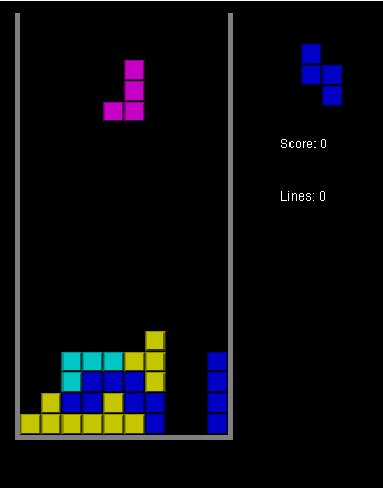
\includegraphics[width=2in]{tetgame.jpg}
\caption{Tetris game in progress}
\label{fig:tetgame}
\end{figure}

Tetris, shown in figure \ref{fig:tetgame}, is so well established that its name has basically lent itself to the entire genre of puzzle games. All variations have a range of different tetrominoes (see Figure \ref{fig:pieces} for the standard set), which are each defined by a static arrangement of square blocks. These tetrominoes can be rotated and translated in the absence of obstructions. 

\begin{figure}[h]
\centering
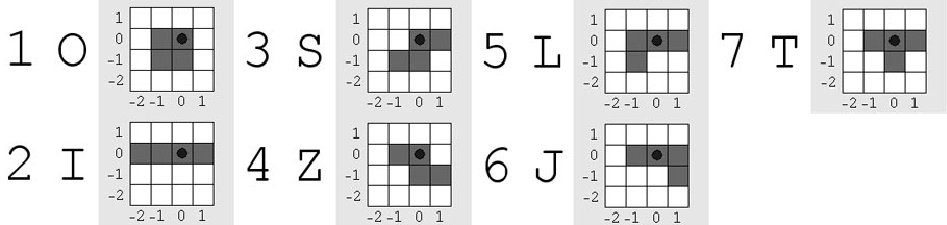
\includegraphics[width=\textwidth]{tetrisblocks.jpg}
\caption{The range of complete Tetris pieces as defined by \cite{tetstand}}
\label{fig:pieces}
\end{figure}
 
A  single tetromino is selected by the game and appears in the top centre block of a fixed-sized discrete well. The tetromino descends at a discrete fixed rate, which is determined by the current difficultly level, until it meets an obstruction. The tetromino is fixed in place if the contact still exists in the descent step following initial contact with an obstruction. If in being fixed it completes a row, the row is completely removed and the entire well's contents above the deleted row are shifted downwards one row.

Many different artificial intelligence approaches have been applied to Tetris, and in order to remove implementation discrepancies when comparing algorithms, guidelines defining the Tetris game must be adopted. The agent, given the successful application of RL, will therefore achieve results which will be directly comparable with those attained by other implementations following the same specifications. The standards set forth by \cite{tetstand} were selected, as there is a fair amount of existing artificial intelligence research associated with them and they seem reasonable, intuitive and comprehensive.

\subsection*{Formal Tetris Specification \citep{tetstand}} 
\begin{itemize}
\item{Tetris has a board with dimensions 10 x 20}
\item{Tetris has seven distinct pieces (See Figure \ref{fig:pieces})}
\item{The current game piece is drawn from a uniform distribution of these seven pieces}
\item{Points are awarded for each block that is landed (not for completing rows)}
\item{The player scores the most points possible for each piece by executing a drop before one or more free-fall iterations transpire}
\item{The game has ten different difficultly settings, which determine the period of free-fall iterations, and are applied as row completion passes certain thresholds}
\end{itemize}

We strictly adopt the first three specifications, but the remaining specifications entail minor adjustments in implementation and only warrant adoption when the agent is contrasted against existing results. We initially remove the time-based descension of the tetromino, since we are dealing with a digital agent whose processing power is machine dependent and we wish to remove scoring discrepancies due to hardware differences.

Artificial intelligence approaches to Tetris are categorised according to the information supplied to the artificial agent. An agent that is solely aware of the current tetromino is referred to as a one-piece algorithm, while an agent that is also informed about the next tetromino is referred to as a two-piece algorithm. An agent that is informed of the next tetromino is given an obvious advantage and can plan its current tetromino placement accordingly. This restricts the comparison of algorithms to other algorithms within the same category.

\section{Mathematical foundations of Tetris}

It has been mathematically proven \citep{mathproof,losetetris} that it is possible to generate a sequence of tetrominoes that will guarantee the eventual termination of any game of Tetris played in a well of width 2(2n+1), with n being any integer. This is most readily achieved by sending alternating Z and S pieces (see figure \ref{fig:pieces}) into the well, which leads to the gradual accumulation of persistent blocks and eventually the termination of the game \citep[Chpt. 5]{mathproof}. The implication of this is: even if the agent were to play a flawless game of Tetris, the series of tetrominoes that guarantees termination of the game is statistically inevitable after a long enough time (infinite period). 

The number of rows completed by a good Tetris player will follow an exponential distribution \citep{tetstand}, owing to the stochastic nature of the game. Some Tetris games are harder than others due to the pieces drawn and the order in which they are delivered, and the resulting performance spectrum can be mistaken for erratic behaviour on the part of the player.

Tetris has also been proven to be NP-complete \citep{hardtet}. The implication of this is that it is computationally impossible to linearly search the entire policy space and select an ideal action. This justifies the use of approximating techniques like RL in trying to determine the optimal policy.

One of the assumptions RL requires is that the environment has the Markov property \citep{suttonbarto}. Tetris satisfies this requirement, as all the relevant information required to make an optimal decision is represented in the state at any instant in time. Rephrased, there is no historical momentum to the current state of the system, and any future occurrence is therefore entirely dependent on the current state of the system. If one is handed control of a Tetris game at any point, one is as equipped to play from that point as one would be had one played up until that point.

\section{Solving NP-Complete problems}

Attractive solutions to problems outside of the computational range of linear search methods can be discovered by emulating biological processes. Two such approaches are genetic algorithms and RL. 

Genetic algorithms search directly in the solution (policy) space of a problem, breeding solutions amongst the fittest individuals in order to approach an optimal solution. RL yields an environment to an agent that is subsequently left to explore for itself. The agent gets feedback directly from the environment in the form of rewards or penalties, and continuously updates its value function towards the optimal policy. Both methods ideally converge on the best policy\citep{evvsrl}, although their different routes gear them towards distinct problems.

RL offers a higher resolution than genetic algorithms, as genetic algorithms select optimal candidates at the population level, while RL  selects optimal actions at an individual level \citep{evvsrl}. Every action taken under a RL policy is judged and driven towards the optimal action in that state, whereas in contrast, genetic algorithms reward complete genetic strains regardless of the behaviour of individual genes within the previous episode. RL also differs from genetic algorithms by indirectly adjusting its policy through the updating of its value function. 

A great deal of information is conveyed in the course of a Tetris game, and RL would enable the agent to capture this information and adapt accordingly.  This would also enable a directed real-time adjustment of the agent's policy, rather than a global adjustment at the end of the game. Another consideration is that as the agent's performance improves, the number of rows completed in a game increases and the lifespan of the agent increases. This does not impact negatively on the reinforcement learning agent as it learns with every move, but has an increasingly large impact on the rate of improvement of the genetic algorithm agent, since its learns with the end of each game. These traits indicate that RL is better suited to solving Tetris than genetic algorithms. 

\section{Reinforcement learning}

RL defines an approach to solving problems rather than offering a rigid specification to be followed through to implementation. It is defined in terms of an agents interaction with an environment. The agent's perception of the environment is encapsulated in a value function which spans every state in which the environment can exist and associates a value with each of these states. This value function is updated upon receiving feedback from the environment as defined by the reward function.

The reward function is statically declared outside of the influence of the agent at the outset of a problem and steers the development of the value function. It is important to note that rewards can be either negative or positive, discouraging or encouraging the agent accordingly. 

The agent follows a policy, derived from the value function by the exploration policy, that maps states to actions and therefore dictates the behaviour of the agent \citep{suttonbarto}.

The goal of the agent is to maximise long-term reward. Its initial behaviour is purely driven by trial and error, but as the agent starts to form an impression about the states, it becomes increasingly important for it to strike a balance between the exploration of unknown states and the exploitation of valuable states \citep{suttonbarto}.

RL can be applied in non-deterministic environments, where taking a certain action within the context of a state does not necessary lead to the same reward or same state transition. It does, however, require that the environment be stationary and that the probabilities of getting a certain reward or transitioning to a certain state remain the same \citep{kaelbling96reinforcement}. For completeness it should be noted that reinforcement learning can be extended to problems that are non-stationary on condition they change slowly. This is achieved by emphasising the importance of recent eperiences over historical ones, and allows the agent to continue learning in a slowly varing task. Tetris is a stochastic game due to the random drawing of the next block. However, it is stationary as the game description remains constant and it therefore satisfies the aforementioned reinforcement learning requirements.

\subsection{The value function \label{sec:valfunc}}

RL is a broad field of research and there are many well investigated approaches which are well suited to specific problem domains. In this paper we adopt TD(0) and Sarsa($\lambda$), which both promise different benefits. TD(0) utilises a state-value table which associates a value with every state in the state space. Sarsa($\lambda$) goes beyond this and references an state-action table which associates a value with every action within a state. The values in both tables are indicative of the long-term reward associated with a particular entry. This entry is a state in the TD(0) agent and it is updated through the use of equation \ref{eq:astates}. In Sarsa($\lambda$) this entry represents a state-action pair and these values are updated using equation \ref{eq:sarsa}

\begin{eqnarray}
\centering
V(s_t) & \leftarrow & V(s_t) + \alpha(r_{t} + \gamma V(s_{t+1}) - V(s_t)) \label{eq:astates} \\
Q(s_t,a_t) & \leftarrow & Q(s_t,a_t) + \alpha(r_{t} + \gamma Q(s_{t+1},a_{t+1}) - Q(s_t,a_t)) \label{eq:sarsa}
\end{eqnarray}

$V(s_t)$ refers to the value of the current state, $V(s_{t+1})$ refers to the value of the next state and $r_t$ refers to the reward received in transitioning from the current state to the next state. Similarly, $Q(s_t,a_t)$ refers to the value of the selected action within the current state, and $Q(s_{t+1},a_{t+1})$ refers to the value of the action taken in the destination state, which is chosen by the policy.

Equation \ref{eq:astates} and \ref{eq:sarsa} state that the value associated with the current state is equal to the current value and a correction factor. This factor is the current value subtracted from the sum of the observed reward and discounted future rewards. The value function therefore incrementally converges on a long-term optimal solution.

The $\alpha$ and $\gamma$ terms dictate the behaviour of the update function :

\begin{itemize}
\item{The $\alpha$ term determines the weighting of the current adjustment in relation to all previous adjustments. A large constant $\alpha$ gives recent value function adjustments a larger influence than historical adjustments. In order to guarantee convergence, this $\alpha$ value must be kept relatively small, and this can be further guaranteed by having the $\alpha$ value diminish over the course of an agent's training.}
\item{The $\gamma$ factor determines the extent to which future rewards affect the current value estimation. The larger the $\gamma$ term, the greater the significance attributed to future rewards. This approach of ``backing up" the values is an example of temporal-difference learning \citep{suttonbarto} and is a way of propagating information about future rewards backwards through the value function.}
\end{itemize}

The value function does not necessarily have to take the form of a table. The value function can be seen as a mathematical function that takes the originating state as input and produces the state with the highest predicted value as output. Rather than storing the values in distinct poisitions within a table, this information is stored in the behaviour of the function. This approach removes the storage requirements of the agent at the expense of encrypting the state information in a convoluted function and is not explored further in this thesis.

\subsection{Eligibility traces}

Learning can be accelerated with the use of eligibility traces which update all state-action pairs following every transition.  This is achieved by assigning a unity weighting to state-action pairs when they are visited and discounting this weighting on every subsequent iteration. These weighting terms allow for recently visited states to adjust their value towards those of their destination states through the multiplication of the current correction factor by the weighting on each state. This is process in shown in equation \ref{eq:sarsaelig}.

\begin{eqnarray*}
\delta & = & r_{t} + \gamma Q(s_{t+1},a_{t+1}) - Q(s_t,a_t) \\
elig(s_t,a_t) & = & 1 \\
 \textrm{for all s,a : } & &  \\
Q(s,a) & \leftarrow & Q(s,a) + \alpha elig(s,a) \delta \label{eq:sarsaelig} \\
elig(s,a) & = & \gamma \lambda elig(s,a)
\end{eqnarray*}

where Q(s,a), $\alpha$ and $\gamma$ refer to the quantities defined in \ref{sec:valfunc}.
elig(s,a) is the weighting associated with a particular state-action pair, $lambda$ is the discounting factor used to adjust the weighting following every update and $\delta$ is the current correction factor.

Eligibility traces can be equally validly applied within the TD approach, resulting in TD($\lambda$). However, we restrict its implementation to the Sarsa agent which has a far larger state space to explore.

\subsection{Exploration}

The agent can possess one of a variety of exploration policies. With a purely greedy policy, the agent will always select the state transition believed to offer the greatest long-term reward. Although this will immediately benefit the agent, it may well fail to find the ideal policy in the long run. 

With an $\epsilon$-greedy method, the agent will select the best state transition the majority of the time and take exploratory transitions the rest of the time. The frequency of these exploratory transitions is determined by the value of $\epsilon$ utilised by the policy. It is possible to vary $\epsilon$, in order to have an initially open-minded agent that gains confidence in its value function as its experience increases over time. 

One problem inherent in the $\epsilon$-greedy approach is that the agent explores indiscriminately and is as likely to explore an obviously unattractive avenue as it is to explore a promising one. An alternative approach is offered by the Softmax approach shown in equation \ref{eq:softmax}. This associates a probability of selection with every possible transition, which is proportional to the the predicted value of that transition. This encourages the agent to explore promising-looking transitions more thoroughly than less promising ones.

\begin{eqnarray}
\centering
P & = & \frac{e^{Q_{t}(a)/\tau}}{\Sigma_{b=1}^{n}e^{Q_{t}(b)/\tau}} \label{eq:softmax}
\end{eqnarray}

The degree to which the estimated value affects the probability of selection is dictated by the $\tau$ term, which is referred to as the temperature. For large temperatures the state transitions become almost equiprobable, while at low temperatures the respective probabilities of selection become more sensitive to value differences between the states.  In the limit as temperature goes to zero, the Softmax policy reduces to the greedy policy.

When a goal has been reached the reward function supplies a reward to the agent.  The value associated with the originating state is adjusted accordingly and this reward is gradually backed up throughout the value function in the wake of the following transitions \citep{suttonbarto}.

\subsection{Existing applications}

reinforcement learning performs very well in small domains, and by using the insight offered by \cite{suttonbarto}, it is fairly simple to create an agent that plays simple games like Tic-Tac-Toe or Blackjack successfully. It has been successfully applied to many sophisticated problems such as :

\begin{itemize}
\item{Packet routing in dynamically changing networks \citep{boyan94packet}}
\item{Robotic control \citep{rlrobotics}}
\item{Acrobot \citep{suttonbarto} }
\item{Chess \citep{baxter98knightcap}}
\end{itemize}

Bellman is cited \citep{suttonbarto} as stating that reinforcement learning suffers from the "curse of dimensionality".  This refers to the exponential increase in the complexity of the system as the number of elements in it increases linearly. This tendency has resulted in relatively few successes in large state-space domains \citep{keepaway}. These successes include : 

\begin{itemize}
\item{RoboCup-Soccer Keep-Away \citep{keepaway}}
\item{Backgammon \citep{tdgammon}}
\item{Elevator control \citep{elevator}}
\end{itemize}

\subsection{Large state space successes}

\subsubsection{TD-Gammon}

 \cite{tdgammon} used reinforcement learning to train a neural network to play backgammon. The program was so successful that its first implementation (Version 0.0) had abilities equal to Tesauro's well established Neurogammon \footnote{Neurogammon was a neural network backgammon player, trained on a database of recorded expert games, who convincingly won the 1989 International Computer Olympiad Backgammon Championship.} \citep{tdgammon}.  More noteworthy is that by Version 2.1, TD-Gammon is regarded as playing at a level extremely close to that of the world's best human players and has influenced the way in which expert backgammon players play \citep{tdgammon}. The unbiased exploration of possible moves and reliance on performance rather then established wisdom leads, in some circumstances, to TD-gammon adopting non-intuitive policies superior to those utilised by humans \citep{tdgammon}.

Backgammon is estimated to have a state space larger then $10^{20}$. This state space was reduced by the use of a neural network organised in a multilayer perception architecture. Temporal difference learning with eligibility traces was responsible for updating the weighting functions on the neural network as the game progressed. 

Another benefit associated with using reinforcement learning methods rather than pure supervised learning methods was that TD-gammon could be (and was) trained against itself \citep{tdgammon}.

\subsubsection{RoboCup-Soccer Keep-Away}

\cite{keepaway} managed to successfully train reinforcement learning agents to complete a subtask of full soccer which involved a team of agents --- all learning independently --- keeping a ball away from their opponents. 

This implementation overcame many difficulties, such as having multiple independent agents functioning with delayed rewards and, most importantly, functioning in a large state space. The state space problem was resolved by using linear tile-coding (CMAC) function approximation to reduce the state space to a more feasible size \citep{keepaway}.

\subsection{Reinforcement in Tetris}

We found three existing extentions of reinforcement learning to Tetris that all use one-piece methods.

\subsubsection{Reduced Tetris}

\cite{melaxtetris} applied reinforcement learning to a greatly reduced version of the Tetris game. His Tetris game had a well with a width of six, an infinite height and the greatly reduced piece set shown in figure \ref{fig:melaxpieces}. The length of the game was dictated by the number of tetrominoes attributed to the game, which was set at 10 000. Although the height of the Tetris well was infinite in theory, the active layer in which blocks were placed was two blocks high, and any placement above this level resulted in the lower layers being discarded until the structure had a height of two. The game kept a record of the number of discarded rows and this was used as a score for the performance of the agent. This approach to scoring resulted in better performance corresponding to a lower score. 

The two block active height prevented the agent from lowering the block structure and completing rows that it initially failed to complete. This differs from traditional Tetris where a player can complete a previously unfilled row after reducing the well structure and re-exposing it. Since the pieces are drawn stochastically and unfilled rows form an immutable blemish on the performance evaluation of the agent, this introduced a random aspect to the results.

The agent was implemented using TD(0) and was punished a hundred points for every level it introduced above the working height of the well.

\begin{figure}[h]
\centering
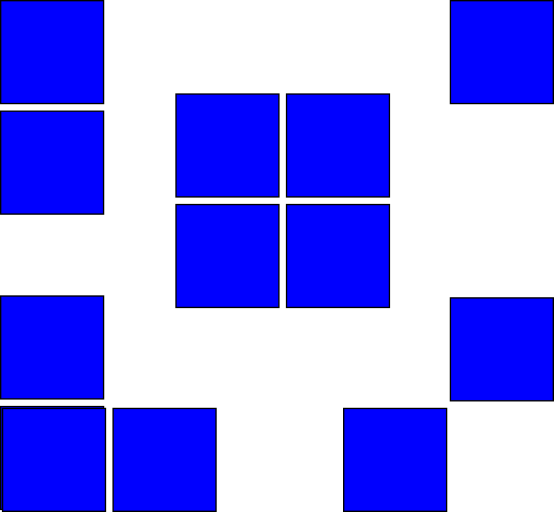
\includegraphics[width=2in]{reducedblocks.png}
\caption{Melax's reduced tetrominoes}
\label{fig:melaxpieces}
\end{figure}

Melax's agent achieved significant learning, as shown in table \ref{mresults}. These results are reflected in figure \ref{fig:meres}.

\begin{table}[h]
\centering
\begin{tabular}{|r|r|}
\hline
Game & Height  \\
\hline
    1 &  1485 \\
     2  & 1166 \\
     4  & 1032 \\
     8  &  902 \\
    16  &  837 \\
    32  &  644 \\
    64  &  395 \\
   128  &  303 \\
   256   & 289 \\
\hline
\end{tabular}
\caption{Melax's results for reduced Tetris}
\label{mresults}
\end{table}

\begin{figure}[h]
\centering
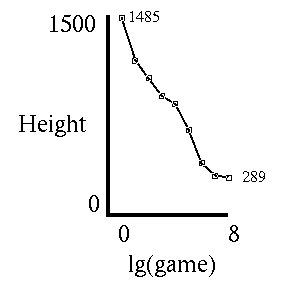
\includegraphics[width=2in]{melaxresults.png}
\caption{Melax's results as taken from \cite{melaxtetris}}
\label{fig:meres}
\end{figure}

As the number of games increased, the agent learned how to minimise the total height of the pieces in the well and therefore maximised its long-term reward.

One possible problem with this implementation is that by defining rewards for sub-goals, such as increasing the working height, the agent is discouraged from a range of policies that may include the optimal policy.  Melax effectively steered the development of the agent's policy towards reducing the height following every transition, rather than placing the blocks optimally and reducing the height of the final structure. Keeping the height of the game low leads to the completion of rows as the agent builds horizontally, and this might actually be the ideal policy for the agent to adopt. However, the optimal policy may never be discovered. This reward structure is ideal in the context of Melax's well description, as the historical well information beneath the working height is discarded and immediate rewards are therefore dominant. What bears consideration is that, with a different well representation, reinforcement learning might achieve a superior optimal policy, and these results reflect on the well representation rather than the reinforcement methods.

\subsubsection{Mirror Symmetry}

Melax's approach was adopted and extended by \cite{yaeltetris}, who investigated different reinforcement learning algorithms and introduced state space optimisations. The state space was reduced through two distinct approaches. In the first approach, subsurface information was discarded leaving only the contour of the game for consideration. This approach was further divided into either considering the contour differences as simply being positive or negative or reducing the height differences to a small spectrum. The second state space reduction made use of mirror symmetry within Melax's well in order to reduce the number of different states.

\begin{figure}[h]
\centering
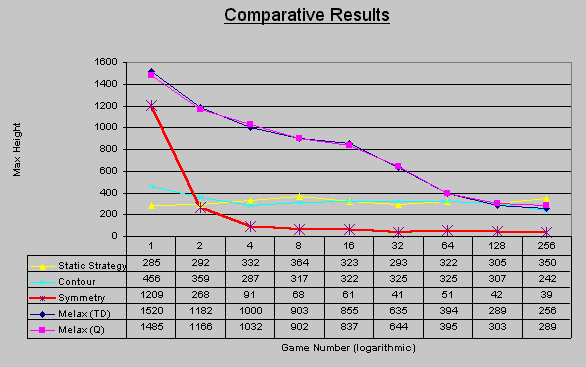
\includegraphics[width=3.5in]{results.png}
\caption{Bdolah and Livnat's results as taken from \cite{yaeltetris}}
\label{fig:yaelres}
\end{figure}

Both optimisations appear to have greatly improved the performance of the agent, judging by the chart shown in figure \ref{fig:yaelres}. There are, however, some troubling aspects to these results.

The mirror symmetry results are far superior to the results achieved by any other method. This optimisation effectively ignored one reflection of duplicated states, and thus should have sped up the learning process while converging on the same solution. The accelerated learning is evident, but the results indicate that the mirror symmetry actually led to the adoption of a distinctly different policy to that adopted by the original agent. This means that the value function must have converged on a different set of values, which negates the original assumption that the values are identical and neccesarily redundant. These results are suspicious, and our own investigation, discussed in chapter \ref{melaxchapt}, reveals the predicted increase in learning speed while converging on the original optimal policy.

The contour learner extended the perceptions of the agent and maintained information below the original two layer structure. This enabled the agent to continually reduce the well structure over the course of the game and therefore reduce the height that was gained. These results seem to indicate incredibly fast learning, and by the end of the first game, the agent settles on a policy that produces a result far superior to the original Melax result.

Despite the dubious results associated with the mirror symmetry optimisation, it is a sound suggestion that is perfectly legitimate in the Tetris game defined by Melax. Incorporating this in the reduction of our final state space would roughly halve the number of states required to describe the Tetris well.

\subsubsection{Relational reinforcement learning}

Relational reinforcement learning was applied to the full Tetris problem by \cite{kurt}. Relational reinforcement learning differs from traditional methods in its structuring of the value function. Rather than storing every possible state in a table, the relationship between the elements in the environment is utilised in developing a reduced state space. This state information is then stored in a decision tree structure. 

Driessens approached the problem with three separate relational regression methods \citep{kurt} that he had developed over the course of his thesis. The first of these regression methods had already proven itself with the successful extension of reinforcement learning to Digger\footnote{Another arcade game with a large state space}. 

Driessens results for full Tetris are shown in table \ref{tbl:driessens} .

\begin{table}[h]
\centering
\begin{tabular}{|r|r|r|}
\hline
Regression method & Learning games & Average completed rows \\
\hline
RRL-TG	&	5000	& 	10   \\
\hline
RRL-RIB  &  50  & 12  \\
\hline
RRL-KBR  &  10-20  & 30-40  \\
\hline
\end{tabular}
\caption{Relational regression results \citep{kurt}}
\label{tbl:driessens}
\end{table}

The RRL-RIB agent reached its optimal policy within 50 training games. In 450 subsequent training games this policy was not improved upon. The RRL-KBR agent reached a better policy earlier than the other regression methods. It then rather unexpectedly unlearned its policy after a further 20-30 games.

Since this is actually a full implementation of Tetris, its results can be compared against other one-piece artificial intelligence methods. The best hand coded competitor completes an average of 650 000 rows per game and the best dynamic agent, utilising genetic algorithms, completes an average of 74 000 rows per game\citep{tetstand}. Driessens results are not impressive in light of the competition and are very poor even by human standards.

Driessens attributes the poor functionality to Q-learning, stipulating that Q-learning requires a good estimate of the future rewards in order to function properly and that the stochastic nature of Tetris severely limits the accuracy of these estimates. Since his regression methods were derived from Q-learning, this inadequacy impacted all of his methods. Q-learning in known to be unstable \citep{keepaway,thrun93issues} when incorporated in function approximation, and this could certainly have contributed to the poor performance shown by the above results.

Despite the final results of Driessens's agent, the idea of exploiting the internal relationships present within the Tetris well as a means of reducing the state space is an attractive one. The change in height between successive columns encapsulates all the information we wish to retain, and since the first position in the well becomes the reference point, the width under consideration is decreased by one.

\section{Conclusion}

This chapter associated the project with a Tetris standard and contextualised the reduction of the Tetris state description performed in the next chapter. Previous Tetris implementations suggested possible state-space optimisations such as using mirror symmetry and relational information. Melax's agent offers credible results for comparrison and a clean specification that was used as an initial reinforcement learning experiment and is discussed in chapter 4. The reinforcement learning concepts covered in this chapter are integral to the implementation of the agent and were directly incoporated into the design of the agent as shown in the next chapter.

\chapter{Design}

In this chapter we reduce the state space of Tetris by adopting assumptions and discuss the possible consequences of each assumption. We then design the reinforcement learning agent and consider the processes it requires. We end the chapter by considering the structure of the whole application.

\section{Redesigning the state space}

Traditional reinforcement learning uses a tabular value function which associates a value with every state. The primary design consideration is how the Tetris state space can be reduced without discarding pertinent information. Since the full Tetris well, shown in figure \ref{fig:fullwell}, has dimensions twenty blocks deep by ten blocks wide, there are 200 block positions in the well that can be either occupied or empty.

\begin{figure}[h]
\centering
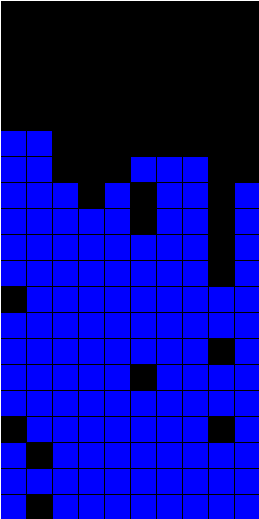
\includegraphics[width=0.8in]{fullwell.png}
\caption{The full Tetris well}
\label{fig:fullwell}
\end{figure}

\begin{eqnarray*}
\centering
\textrm{State Space} & = & 2^{200} 
\end{eqnarray*}

This is an unwieldy number and since a value would have to be associated with each state, this representation is completely infeasible. We choose to stick with traditional reinforcement learning and introduce reductions in the tabular description of the environment by considering the game from a human perspective and by adopting the mirror symmetric optimisations suggested by \cite{yaeltetris}. 

\subsection*{Assumption 1}

The position of every block on screen is not a consideration that is factored into every move by a human player. We only consider the contour of the well when making decisions. We limit ourselves to merely considering the height of each column.

\begin{figure}[h]
\centering
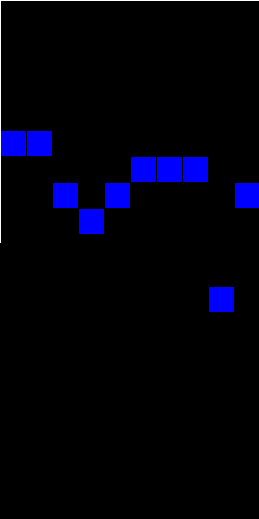
\includegraphics[width=0.8in]{heightwell.png}
\caption{Height-based Tetris well}
\label{fig:heightwell}
\end{figure}

\begin{eqnarray*}
\centering
\textrm{State Space} & = & 20^{10} \approx 2^{43}
\end{eqnarray*}

\subsection*{Assumption 2}

The height of each column is fairly irrelevant except perhaps when the height of a column starts to approach the top of the well. The importance lies in the relationship between successive columns, rather than in their isolated heights.

\begin{figure}[h]
\centering
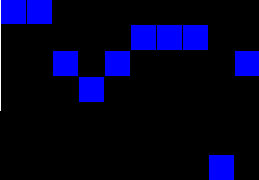
\includegraphics[width=1.6in]{diffheightwell.png}
\caption{Height difference-based Tetris well}
\label{fig:diffheightwell}
\end{figure}

\begin{eqnarray*}
\centering
\textrm{State Space} & = & 20^{9} \approx 2^{39}
\end{eqnarray*}

\subsection*{Assumption 3}

Beyond a certain point, height differences between subsequent columns are indistinguishable. A human will not adopt different tactics when the height difference between two columns advances from nineteen to twenty. We could either cap the maximum height differences or start separating the heights into fuzzy sets as the height differences increase past certain thresholds. We cap the maximum height difference between wells at $\pm$ 3, and truncate all height differences outside of this range down to $\pm$ 3. The agent will therefore generalise for any height difference greater than three. Since only the straight tetromino can span a height difference of three, and this tetromino can span any height difference, this assumption seems fair to make. 

\begin{figure}[h]
\centering
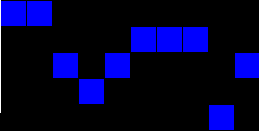
\includegraphics[width=1.6in]{capdiffheightwell.png}
\caption{Capped height difference-based Tetris well}
\label{fig:capdiffheightwell}
\end{figure}

\begin{eqnarray*}
\centering
\textrm{State Space} & = & 7^{9} \approx 2^{25}
\end{eqnarray*}

\subsection*{Assumption 4}

The largest tetromino is four blocks wide. At any point in placing the tetromino, the value of the placement can be considered in the context of a subwell of width four. These subwells could then be extended to the full well by tiling them across the extent of the full well.

\begin{figure}[h]
\centering
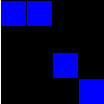
\includegraphics[width=0.8in]{reducedwell.png}
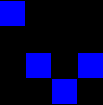
\includegraphics[width=0.8in]{reducedwell2.png}
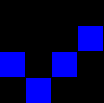
\includegraphics[width=0.8in]{reducedwell3.png}
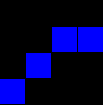
\includegraphics[width=0.8in]{reducedwell4.png}
\caption{Capped height difference-based Tetris subwells}
\label{fig:redwell}
\end{figure}

\begin{eqnarray*}
\centering
\textrm{State Space} & = & 7^{3} = 343 \approx 2^{8}
\end{eqnarray*}

\subsection*{Assumption 5}

Since the game is stochastic and the tetrominoes are uniformly selected from the tetromino set, the value of the well should be no different to its mirror image.

\begin{figure}[h]
\centering
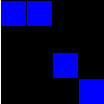
\includegraphics[width=0.8in]{reducedwell.png}
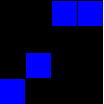
\includegraphics[width=0.8in]{mirrorwell.png}
\caption{Mirror identical states}
\label{fig:mirrorwell}
\end{figure}

\begin{eqnarray*}
\centering
\textrm{State Space} & = 175
\end{eqnarray*}

\subsection*{Repercussions}

We now have a much reduced state space, which we hope will neither limit the agent nor appreciably steer its policy. We subsequently refer to any agent that functions within this state space as a contour agent. The implications of the assumptions adopted above should be considered before we proceed towards implementing the agent that adopts this state representation.

\begin{itemize}
\item{Assumption 1 discards all information about the subsurface structure of the well. The initial representation can be perceived to store the location of every hole in the structure. The agent will therefore be oblivious to any differences between transforming to a said contour and the same contour with spaces beneath the surface. The existing holes are not important, but we may wish to include a penalty for the holes introduced during a state transition.}
\item{Assumption 2 introduces no obvious evils.}
\item{Assumption 3 removes the agent's ability to distinguish between extremes in height differences. It is reasonable to assume that the agent will have to utilise states with large height differences at some point in following the optimal policy, and that the storing of states with large and extreme height differences within the same value may lead to the agent acting unintelligently in these circumstances. These extreme height states will almost certainly have relatively small values associated with them. Consequently we expect the agent to generally avoid selecting states with large height differences, even if selecting the state would follow the true optimal policy.}
\item{Assumption 4 removes the global context in which the agent functions and restricts its view to each individual transition. We will need to dynamically re-establish the context in which it is functioning, and we deal with this in Chapter 6.}
\item{Assumption 5 reduces the state space in a non-trivial fashion. The mirrored states are still allocated space but are never explored, removing the computational burden they represent.}
\end{itemize}

\section{reinforcement learning agent}

We set out to create an agent that functions within the reduced state representation developed above. We decided to implement a one-piece algorithm and the agent can therefore only consider the tetromino currently allocated to it in the course of each move. The agent's behaviour can be separated into distinct processes.

\begin{enumerate}
\item{Discover transitions}
\begin{enumerate}
\item{Calculate index}
\end{enumerate}
\item{Correct for multiple subwells (Note: only used in extending the well) }
\item{Choose amongst transitions using exploration policy}
\item{Update value function}
\end{enumerate}

These processes are now explored as distinct methods. 

\subsection{The discovery of transitions}

This method discovers the transitions available from the current state. The agent makes use of a virtual game that exists purely for its benefit, isolating any conceptual manipulations from the full game. The agent copies the block formation from the real Tetris well into its virtual well before performing each of the possible transitions with the current tetromino. The well structure resulting from each transition is used by the indexing function to calculate the appropriate index into the value function. Each transition is stored as an object that contains the number of translations and rotations, the resulting reward and the value of the resulting state.  Every unique transition is then added to the list of possible transitions.

\subsection{The calculation of indexes}

An indexing function in used to associate every Tetris state with a unique position in the value table. The indexing function is completely dependent on the state representation of the game and therefore differs from the Melax-defined agent developed in Chapter 4 and the agent we develop in Chapter 5.

For the Melax-defined agent, the well is viewed as a 12 block array. The first position is assigned a value of one, and this value is doubled for each successive block position. If the position is occupied, the value of that position is added to an accumulator. This enables us to calculate a unique index for every state through the use of addition.

For our contour agent, the well is viewed as a block array one block narrower than the well the agent is playing in. Each of these positions can have a value between 0 and 6, corresponding to a height difference of -3 and 3 accordingly. The first position is assigned an intrinsic value of 1. The intrinsic value of each subsequent position is determined by multiplying the previous position's intrinsic value by 7. Multiplying the values in the block array by the intrinsic value of the array position and summing the resulting products yields a unique index. This method is not limited to height differences of 7 and is readily expandable, with the inherent values of the block positions increasing as $x^n$, where $x$ is the number of height differences and $n$ the relative row position.

\subsubsection{The index adjustment due to mirror symmetry}

Mirror symmetry is factored into both of the above indexing functions by calculating the index values from both directions. The smallest value is then always selected. The unused array positions are still issued storage space but are never explored, and they therefore introduce no exploratory overhead.

\subsubsection{The index adjustment due to further extentions in the game description}

The above indexing functions solve the problem of representing the state space. Expanding the agent's perception beyond the state is handled by introducing an adjustment to the previous calculated index. This index adjustment function adds further weighted terms to the existing index. The weighting used is always the full size of the previous state description. Sarsa for instance requires state-action value tables. The state index is adjusted to include the tetromino type, position of placement and number of rotations. Each enhancement adds the existing index to the new consideration multiplied by the existing state space.

This approach facilitates the continued expansion of the state description. 
 
\subsection{Correcting for multiple subwells}

We solved the disparity between the full Tetris well and the contour Tetris well by breaking the full well into overlapping subwells. This is shown in figure \ref{fig:subwells}.

\begin{figure}[h]
\centering
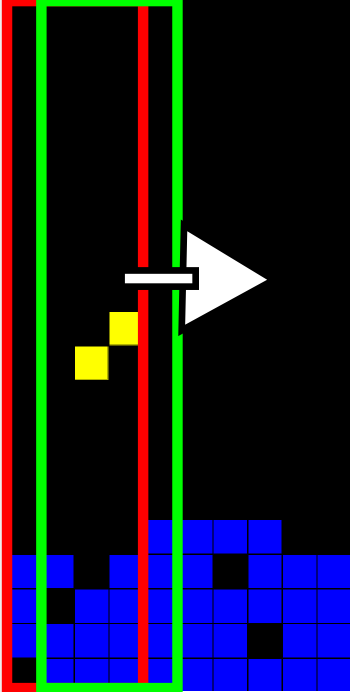
\includegraphics[width=1.2in]{decomposedwell.png}
\caption{Dividing of well into subwells}
\label{fig:subwells}
\end{figure}

In discovering possible transitions, the agent previously iterated through every possible positional placement and every orientation of the current tetromino within these placements. In extending the subwell representation to the full game, the agent had to iterate through all the subwells comprising the full well and investigate the value of the transitions in the subwells.

These subwells are identical to the wells in which our agent trained throughout the previous chapter. Every transition in every subwell is considered and a global transition is then selected. There were two distinct approaches to selecting global transitions out of all the subwell transitions. The subtransitions occupying the same physical description in the full well can be averaged, leading to a single transition which reflects the value of the transition across all the subwells and gives a broad overview of the value of the transition. Another approach is to retain the largest transition value from all the subwells, disregarding all the other transitions and placing the emphasis on selecting the optimal action.

The transitions in the full well are therefore related to transitions in the subwells by a transition adjustment function which accepts the complete range of subtransitions and returns a list containing a single value for every transition in the full well.

\subsection{Exploring amongst transitions}

$\epsilon$-greedy, greedy and softmax are implemented as competing exploration policies, and any of them can be implemented alongside optimistic learning if desired.

Greedy and softmax are implemented as distinct policies. However, $\epsilon$-greedy is a deviation from the greedy policy and is implemented within the greedy method by giving the agent a fixed probability of choosing randomly amongst the available transitions. There are therefore two methods that accept a range of possible transitions and return a single transition.

Optimistic learning is achieved by initialising the value function with values slightly larger than the largest anticipated value. This value is easily determined when dealing with purely negative rewards, since all states will have negative values and therefore zerp is an optomistic value. When dealing with positive rewards, the easiest approach is to set the agent to explore for a large period of time, look at the predicted values and adopt a value slightly larger than the largest value for the starting values.

\subsection{Updating the value function}

The transition selected by the exploration policy is then taken in the full game. The results of this transition are used in updating the agent's value function.

The update functions for the TD(0) and Sarsa($\lambda$) agents are shown by equation \ref{eq:astates} and \ref{eq:sarsaelig}, respectively. The two approaches require different state representation and data manipulations, and this disparity is grounds for implementing distinct agents. 

The update method accepts the current index, destination index and a reward. In the Sarsa($\lambda$) agent this reward is interpreted as the reward associated with taking the action from the current state. In TD(0), the reward can be interpreted as the reward received in transitioning from the current state to the destination state.

In implementing the Sarsa($\lambda$) agent, the value table had to be extended to contain every transition off each state. The number of transitions is dictated by the number of different tetrominoes, the width of the well and the number of different orientations.  The size of the state-action space is calculated by multiplying the number of transitions by the original number of states. This drastically increases the state space of the game and may introduce a great deal of redundant information depending on the tetromino set used. Fixing this would require including tetromino-set specific considerations in our Tetris implementation and would remove the generic nature of the implementation. We choose to retain the redundancy as, although it introduces additional training time, it should not impact the final values converged on by the value function.

Replacement eligibility traces are implemented in the Sarsa($\lambda$) update method. 

\section{Application design}

We designed a Tetris game from first principles in order to have complete control over the structure of the game and familiarise ourselves with the required methods.

The application can be readily divided up into the following logical classes.

\begin{itemize}
\item{The game window}
\item{The Tetris game}
\item{The tetromino set}
\item{The tetromino object}
\item{The tetris player}
\end{itemize}

The interaction between these components is shown in figure \ref{fig:uml}

\begin{figure}[h]
\centering
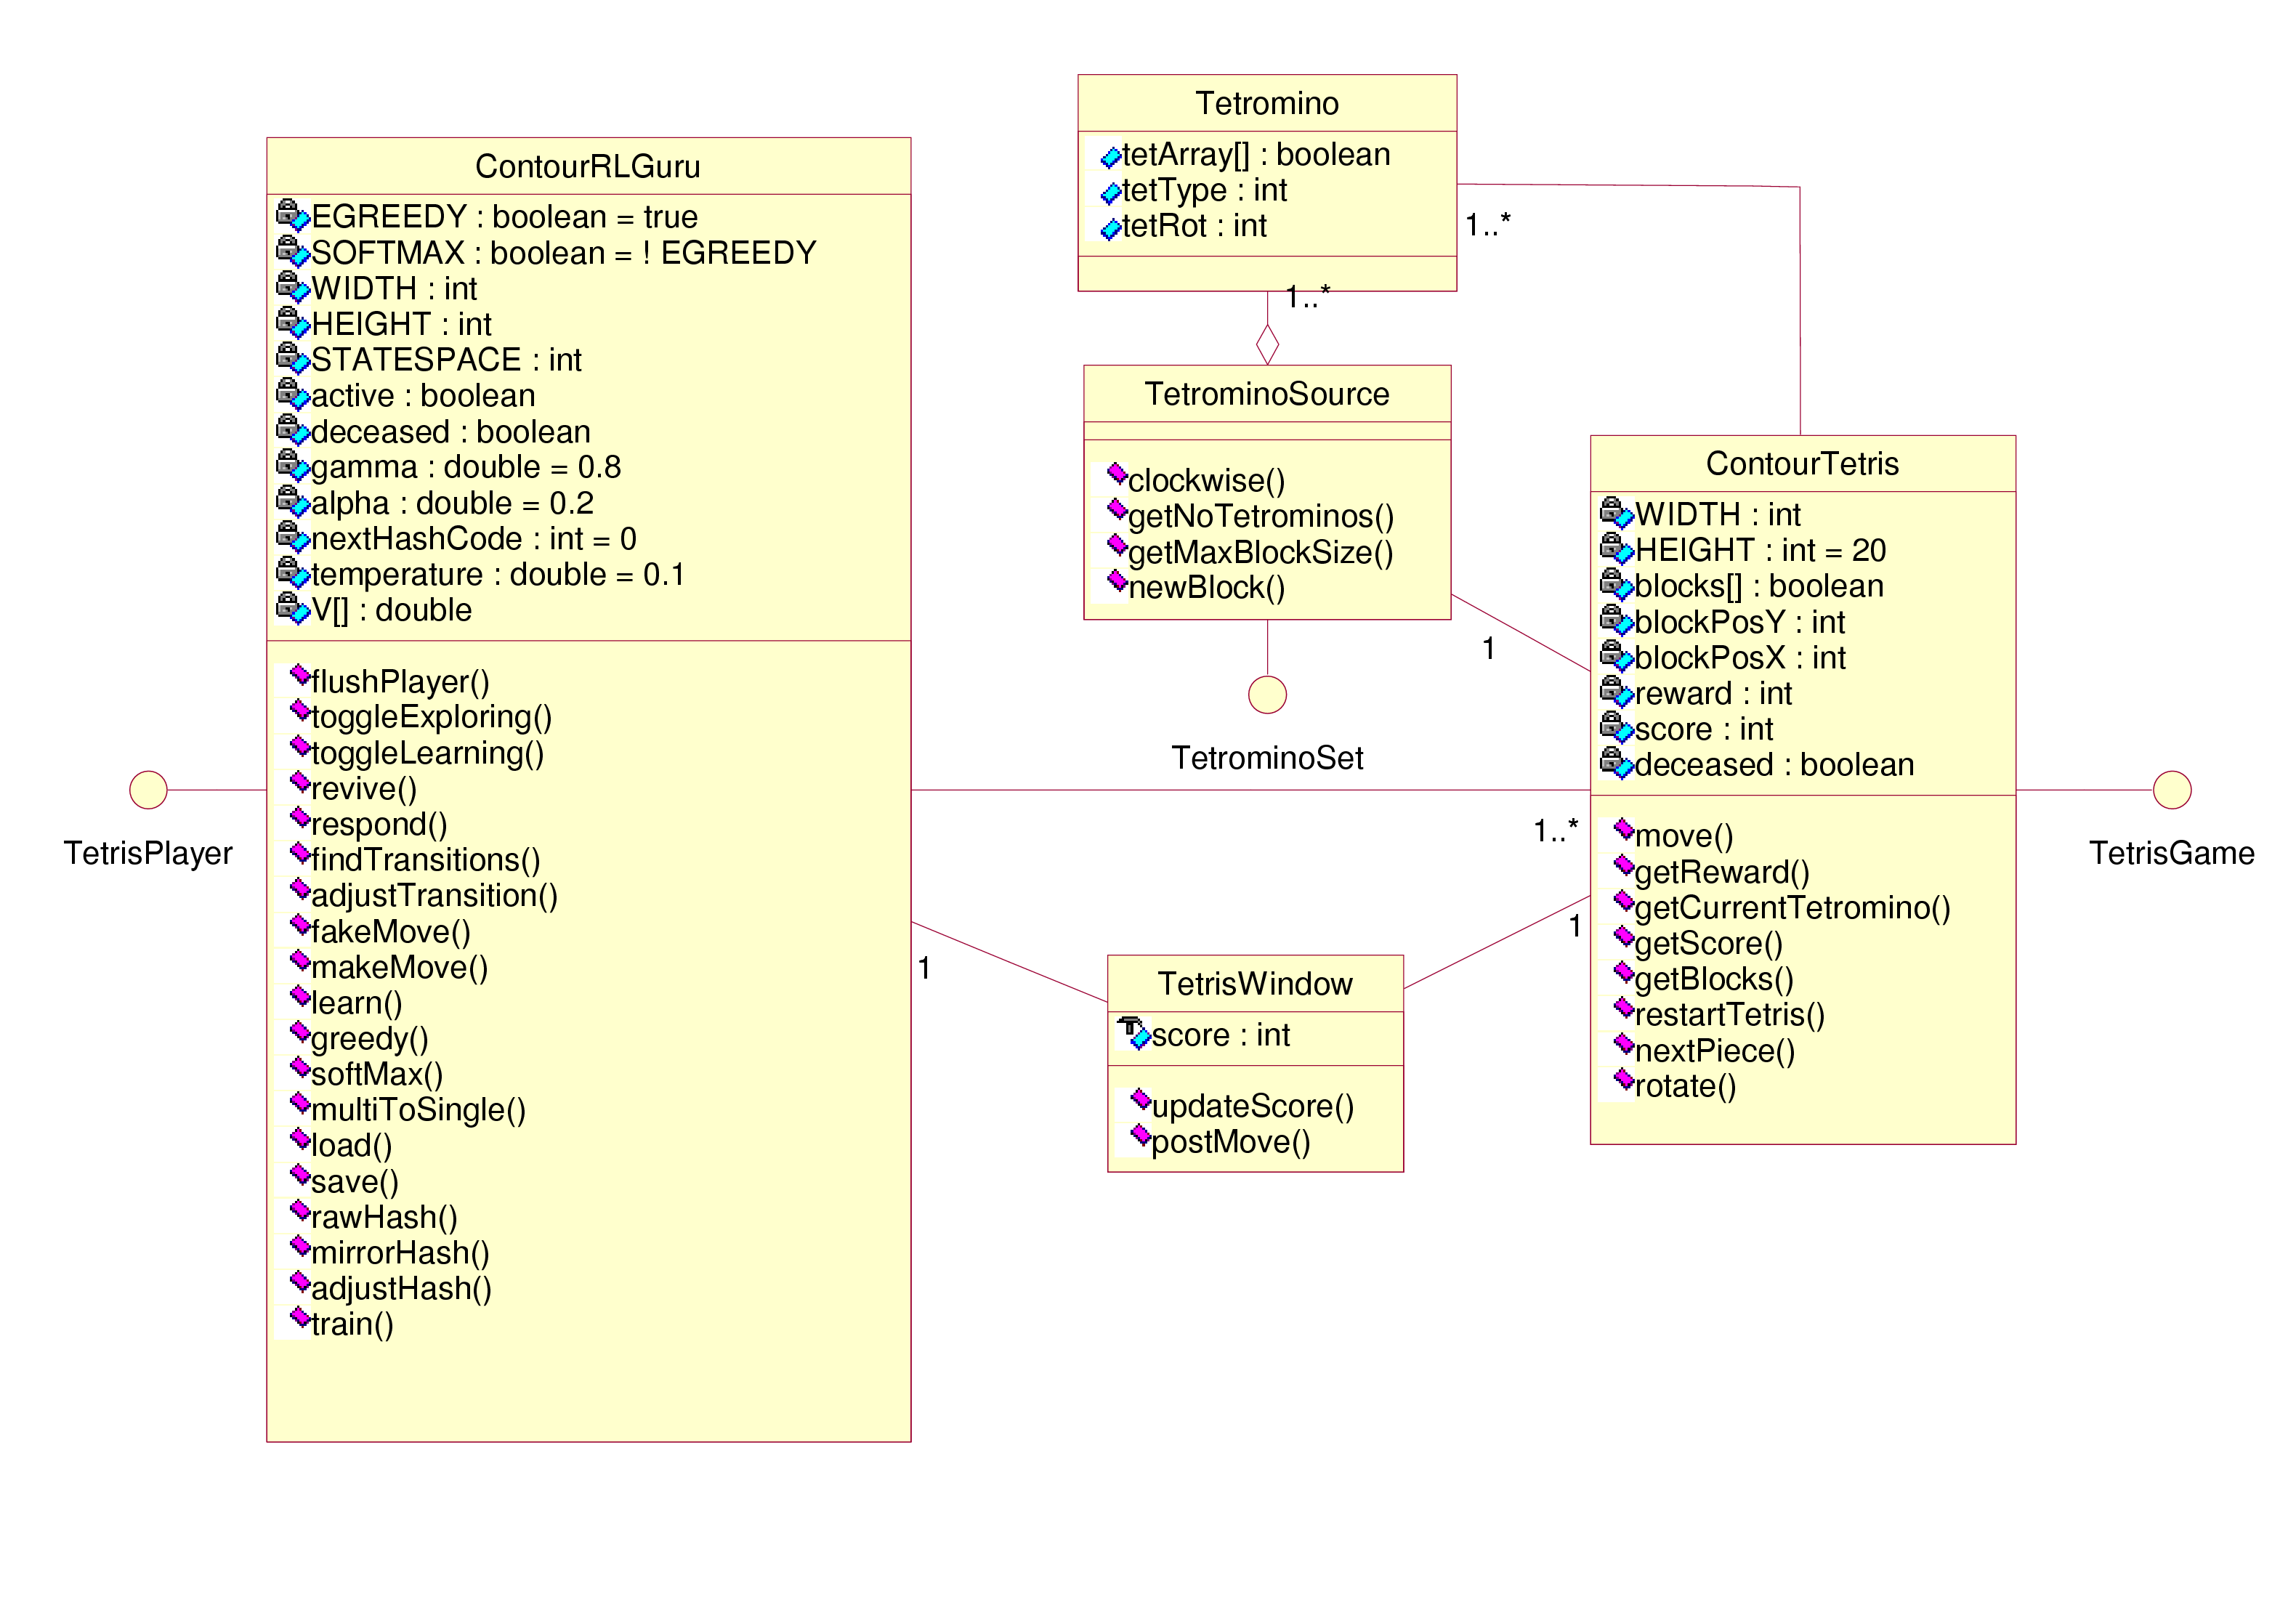
\includegraphics[width=6in]{finaluml.png}
\caption{Class diagram of reinforcement leaning oriented Tetris}
\label{fig:uml}
\end{figure}

The game window acts as the interface between the user and the Tetris game, and is responsible for displaying all information regarding the system. The Tetris game is the self-contained core of the program and is responsible for managing the game and yielding information on the state of the game. The Tetris game and agent are both instantiated in the game window and the agent is passed a reference to the game upon instantiation. Exclusive control is switched between either of these two control sources, and the game is therefore oblivious to the source of its instructions.  Including human interaction enables the Tetris implementation to be checked. The tetromino set is instantiated within the Tetris game and is responsible for the definition and rotational manipulation of the tetrominoes. All tetromino transitions which occur within the well are checked and performed in the Tetris game. The tetromino object is common to all methods and is a simple structure encapsulating the traits of a tetromino. This object is oblivious to the definitions dictated by the tetromino source and is used by all the classes.

The Tetris game, tetromino set and the artificial agent are all objects that will need to change in the course of the investigation. This is simplified if these three objects implement generic interfaces which allow us to utilise polymorphism. This structuring allows for seamless swapping between different game definitions, tetromino sets and artificial agents. The differing game definitions are largely restricted to variations in the dimension of the well, whereas tetromino-set definitions are unrestricted and any tetromino collection can be created. As long as the agent implements the correct interface, the theory guiding the actions of the agent can subscribe to any artificial intelligence method. This follows the reasoning, outlined by the strategy design pattern \citep{designp}, that competing algorithms should implement a common interface and therefore be seamlessly interchangable.

We would expect any object-orientated Tetris game to deal with a large number of tetromino objects, and the performance penalty introduced by instantiating large numbers of simple objects warrants consideration. This is addressed by conventional design patterns and corresponds to a fly-weight pattern, as discussed in \cite{designp}. Rather than having the game continually recreating individual tetrominoes within the set of available tetrominoes, it is preferable to create every possible tetromino once and subsequently pass out a reference to the relevant tetromino. This optimisation is piece-specific and is implemented in the tetromino source class by instantiating a two dimensional array of tetrominoes corresponding to the range of rotations for every tetromino. The first time a tetromino is assigned or uniquely rotated it is created within this array structure, and a pointer is returned following all subsequent requests for this orientation of the tetromino.

\section{Conclusion}

This chapter detailed the design of the reduced well structure we wish to investigate with our agent. The structure of the agent and the processes required by reinforcement learning were discussed in detail. The chapter ended with our addressing the design requirements of a flexible Tetris application. 

\chapter{The Melax-defined player}

In this chapter we implemented our first reinforcement learning agent by following Melax's approach. We investigated the TD(0) value function, the constants utilised in it and a range of exploration methods. We also investigated the effect of including the mirror symmetry optimisation and implemented an agent using Sarsa(0).

\section{Melax Tetris \label{melaxchapt}}

Melax clearly defined the conditions under which his player functioned:

\begin{itemize}
\item{Well has infinite height}
\item{Well has a width of 6 blocks}
\item{The game has a working height of 2 blocks --- any blocks below this are discarded}
\item{The game is limited to 10 000 tetrominoes}
\item{The game uses a reduced tetromino set (See figure \ref{fig:melaxpieces})}
\item{The alpha and gamma values are defined as 0.02 and 0.8, respectively}
\end{itemize}

Melax did not stipulate the exact reinforcement learning approach he applied to his agent, although the update function stated in \cite{melaxtetris} corresponds to a TD(0) update function. Optimistic learning was employed and the initial value estimates for each state were set to zero, which is optimistic when receiving purely negative rewards. The performance of the agent is gauged by the final height of the tetromino structure in the well. The lower the structure height, the more tightly the tetrominoes are packed and the better the performance of the agent.

We followed the Melax specifications and implemented the agent shown in figure \ref{fig:mymelax}.

\begin{figure}[h]
\centering
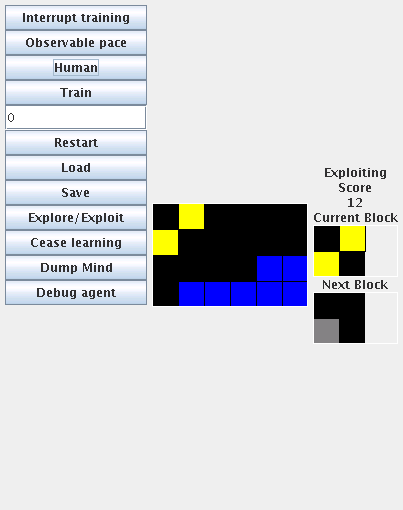
\includegraphics[width=2in]{mymelax.png}
\caption{Our Melax-defined agent}
\label{fig:mymelax}
\end{figure}

\section{Initial Melax results}

The agent was set to exploit its knowledge from the outset (greedy policy) and therefore had to rely on the optimistic initialisation values to inspire its exploration. The results are shown in figure \ref{fig:mymelaxresults} and contrast the performance of our reinforcement learning player to other standards. 

\begin{figure}[h]
\centering
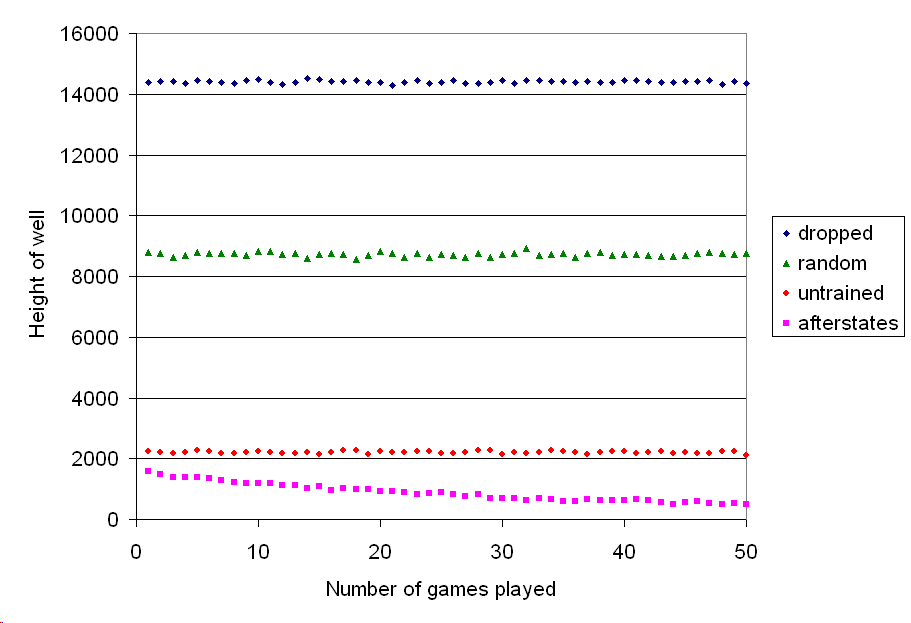
\includegraphics[width=3.5in]{mymelaxresults.png}
\caption{Results for the Melax-defined agent}
\label{fig:mymelaxresults}
\end{figure}

The first standard is the maximum height of the structure and is determined by piling up tetrominoes without undertaking any translation or rotation. The second standard is the height of the structure when the blocks are randomly placed. The final standard is the performance of the agent when learning is switched off before any training has occurred, and the agent is set to exploit its knowledge. As can be seen, the agent has a fair amount of insight into the game through the real time value contribution utilised in TD(0).

The agent starts at the level of the untrained agent and rapidly improves. The height of the well stabilises at a height which is roughly a quarter of the height of the untrained agent.

\section{Mirror symmetry}

We proceeded to implement the mirror symmetric optimisation of the Melax state space identified by \cite{yaeltetris}. Figure \ref{fig:comparemelax} shows the improvement in the agent's performance when the mirror symmetry optimisation is included in the state description. Since all the mirror symmetrical states reference the same position in the table, these values are updated twice as often as they were before the optimisation. This leads to the tabular values converging on the correct values more rapidly. This is clearly reflected in the graphed results, and it is important to note that the final policy arrived at is the same in both circumstances. This vindicates the assumption that mirror identical states should have the same value associated with them and experimentally reinforces the scepticism shown in Chapter 2 when interpreting the results of \cite{yaeltetris}. 

\begin{figure}[h]
\centering
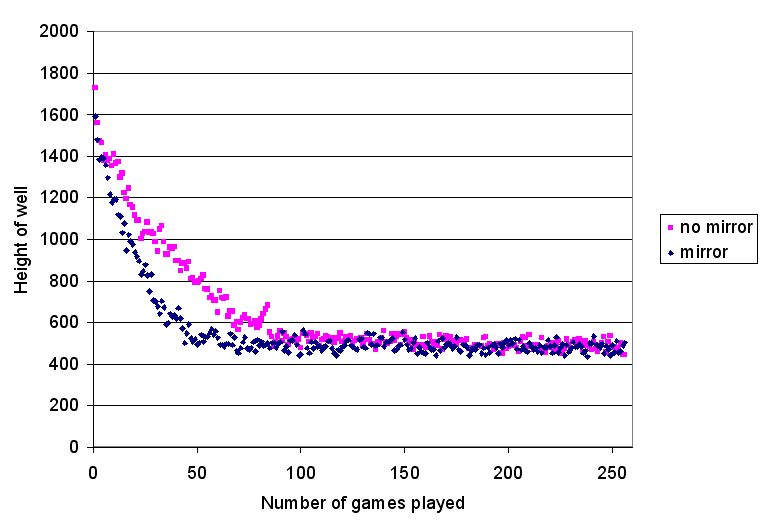
\includegraphics[width=3.5in]{mirrormelax.png}
\caption{Performance impact of mirror symmetry}
\label{fig:comparemelax}
\end{figure}

\section{Different exploration policies}

We used our Melax agent to compare its performance when using the different exploration methods. The different exploration methods are tested with and without optimistic learning and the results are shown in figures \ref{fig:compexpopt} and \ref{fig:compexp}, respectively.

The $\epsilon$-greedy method is set to explore 5 percent of the time. Setting the Softmax parameters introduces difficulties as the initial temperature, rate of change of temperature and final temperature must all be set.

\begin{figure}[h]
\centering
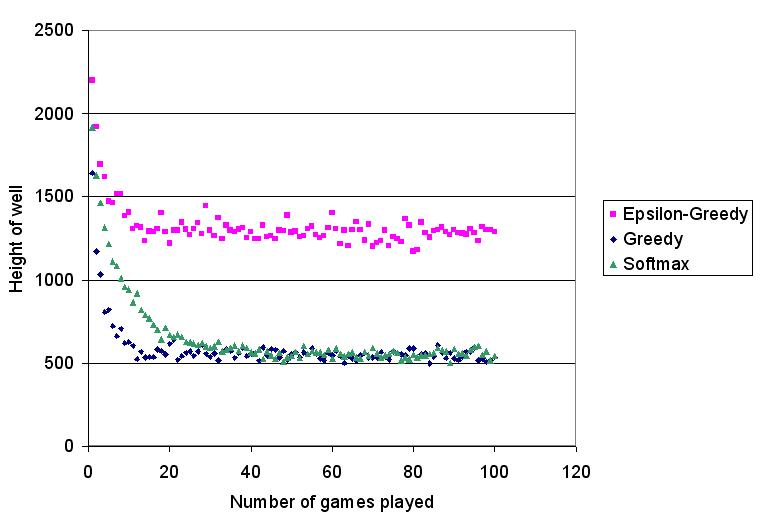
\includegraphics[width=3.5in]{optomisticexp.png}
\caption{Different exploration methods with optimistic learning}
\label{fig:compexpopt}
\end{figure}

Both the greedy and Softmax approaches discover the optimal policy and settle on it. The $\epsilon$-greedy method is never set to exploit its knowledge and taking a random move 5 percent of the time restricts it to achieving a consistent well height of around 1300 blocks. The greedy policy converges on the optimal policy most rapidly as is expected when utilising optimistic learning.

\begin{figure}[h]
\centering
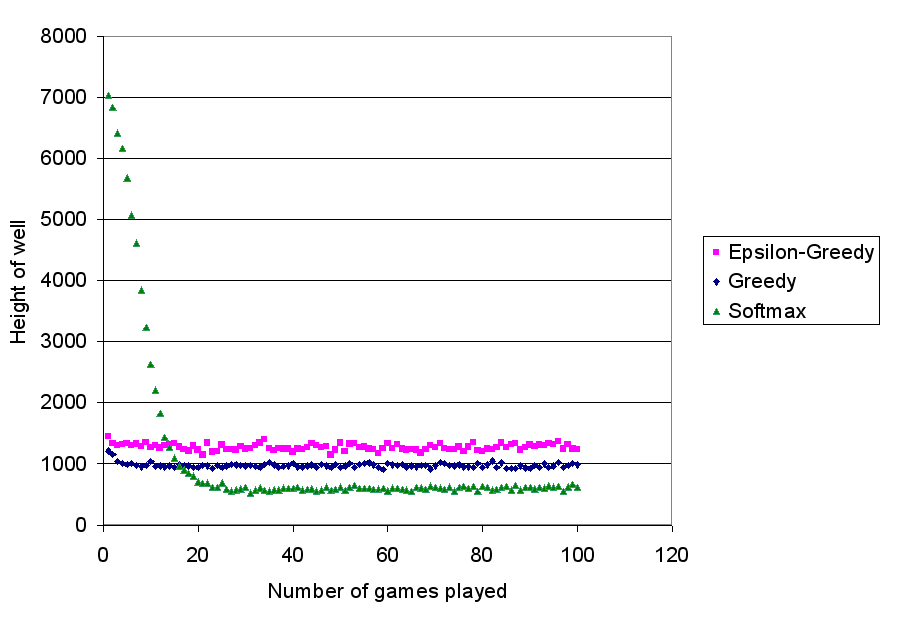
\includegraphics[width=3.5in]{nonoptomisticexp.png}
\caption{Different learning methods without optimistic learning}
\label{fig:compexp}
\end{figure}

The value table of the previous optimistic agent had a minimum value greater then -150 after settling on the optimal policy. The starting values of the non-optimistic agent were therefore set to -150, and the exploration methods were then tested.

The $\epsilon$-greedy agent stumbles upon nothing useful in the training period, and shows absolutely no learning over the investigation period. The greedy player stumbles on to a sub-optimal policy after less then 5 games, and then shows no further improvement following this. The Softmax player shows incredibly rapid learning and settles on the optimal policy within 30 games. The initial height of the well is due to the initially indiscriminate exploration on the part of the Softmax agent.

The Softmax approach proves its worth both with and without the aid of optimistic learning. The drawback with Softmax is that the implementation differs between the optimistic and non-optimistic testcases. Achieving ideal exploration requires discovering the optimal starting temperature, change in temperature and rate of change of temperature. The agent requires the full training period to explore between adjustments to the parameters, and as the state space gets larger the ideal values get increasingly vague and non-tangible. As the state space grows and the agent takes longer to explore, the iterative discovery of ideal learning parameters get progressively more painful.

The combination of optimistic learning and the greedy approach results in the agent learning incredibly rapidly and settling on the optimal solution. A further benefit is that the learning method requires no adjustments with a change in state space and the only quantity that has to be established in the optimistic starting value.

Due to the convenient nature of optimistic learning with the greedy policy we utilised optimistic learning and adopted a greedy policy in all future investigations.

\section{reinforcement learning constants}

Melax found that the optimal policy was discovered with a $\gamma$ term of 0.8 and an $\alpha$ term of 0.02. Through experimentation we discovered that increasing the $\alpha$ term to 0.2 increased the speed of learning by an order of magnitude as shown in figure \ref{fig:alpha}. Adjusting the $\gamma$ term had far less tangible results, and since this shifts the relationship between successive states it can have subtle consequences.

\begin{figure}[h]
\centering
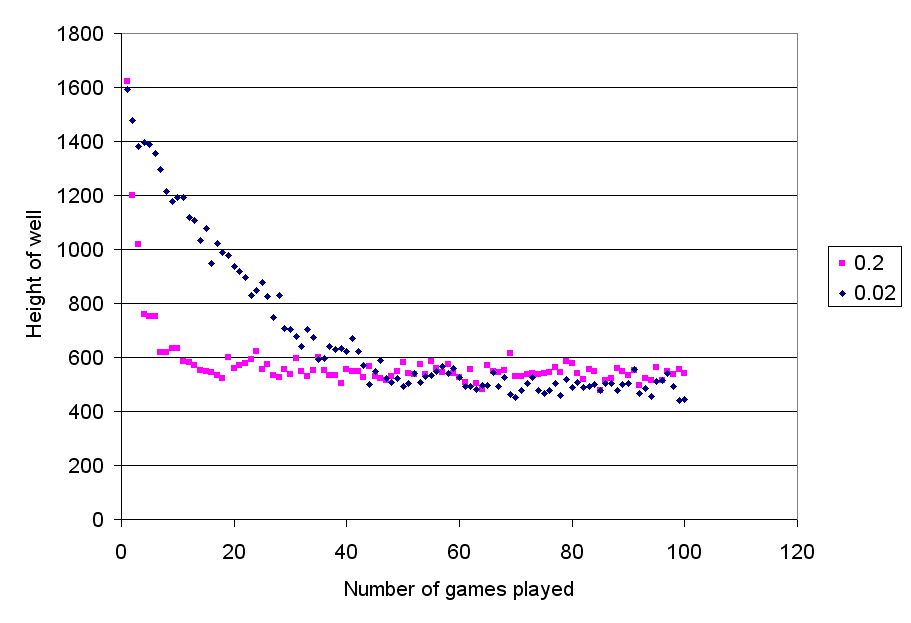
\includegraphics[width=3.5in]{alphacomp.png}
\caption{Impact of $\alpha$ on learning}
\label{fig:alpha}
\end{figure} 

The agent with an $\alpha$ value of 0.02 finally converges to a superior optimal policy, but the improvement in performance is small in proportion to the overall learning exhibited and the increase in training time is a serious drawback.

In all subsequent investigations we maintained an $\alpha$ value of 0.2 and a $\gamma$ value of 0.8 unless otherwise stated.

\section{Sarsa($\lambda$) agent}

Melax mentions having implemented a Sarsa agent without eligibility traces (Sarsa(0)) and reports no appreciable differences in the results achieved by the agent. 

In adopting Sarsa(0) we have to expand the state space. Melax's reduced piece set contains 5 different tetrominoes, the well is 6 blocks wide and any grid based game is restricted to 4 orientations. There are therefore approximately 5*6*4 transitions off each state and the size of the state space is increased from 4096 states ($2^{12}$) to 491520 states (approximately $2^{19}$). The impact of this is that the Sarsa(0) agent takes an incredible amount of time to train as the results in figure \ref{fig:melaxsarsa} show.

\begin{figure}[h]
\centering
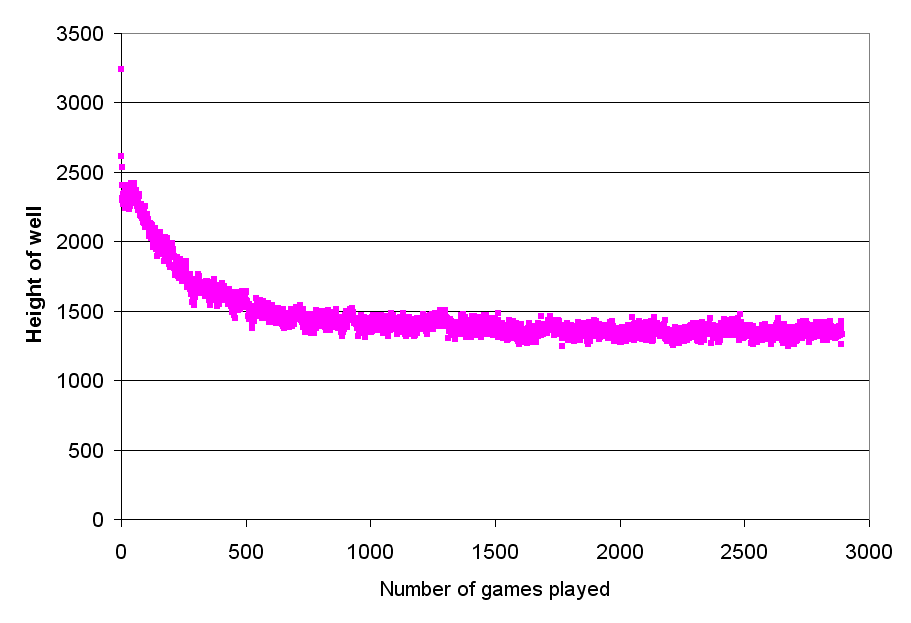
\includegraphics[width=3.5in]{sarsamelax.png}
\caption{Performance of Sarsa(0) agent}
\label{fig:melaxsarsa}
\end{figure} 

A large amount of this exploration time is wasted exploring redundant states, since only the L shaped Melax tetromino has 4 unique orientations, while all the others only have 2 unique orientations. There is further storage wastage as only the single block tetromino can move across the full span of the well regardless of the orientation of the block. 

After learning plateaus off the agent is capable of constructing a well structure around 1400 rows high. These results are far worse then those achieved by the TD(0) agent. The afterstates agent only takes 50 games to find the optimal policy in contrast to the Sarsa(0) agent who takes around 800 games. This increase in training time was expected with the expansion of the state space, but the poor final results are not easily explained. Observing both agents play does not reveal any obvious short sightedness on the part of the Sarsa(0) player.

The Sarsa($\lambda$) agent has all the state information available to the TD(0) agent, and increased perception since it develops a value for every action. It does lack the real time guidance given to the TD(0) agent, and this is only possible source of ignorance we can identify. The approaches are quite distinct, with the Sarsa($\lambda$) relying on purely on its state-action table while the TD(0) agent uses its value table as a supplement to real time information. This task may simply be suited towards the latter approach.

Another possibility is that given enough training time, the agent might have experienced a discontinuous jump in performance and discovered the optimal policy the TD(0) agent is using. This type of performance jump is evident in later agents, and the sheer size of the state space may have prevented the agent from stumbling onto this within a reasonable period of time. (1 full day of training)

\section{Conclusion}

In this chapter we discussed the learning achieved by the reinforcement learning player defined by Melax and discussed the results of further experimentation with the value function constants, mirror symmetry, exploration methods and a Sarsa(0) agent. The results determined in this chapter set many experimental parameters used in subsequent investigations, such as the value of $\alpha$ and the use of the optimistic-greedy exploration policy.

\chapter{Contour Tetris}

The implementation of the Melax agent supplied a great deal of insght in applying reinforcement learning to Tetris, which we used in implementing two agents using the state representation designed in chapter 3.  These agents use TD(0) and Sarsa($\lambda$) respectively and we discuss the performance of our agents with the mind to extend them to the full well.

\section{General}

In creating our agent we had to decide on a reward policy. Initially we wanted to lead the player as little as possible and afford the player the freedom to determine its own policy. Melax's punishing of the agent for increasing the height seemed too prescriptive, and we initially opted to rather reward the agent for simply completing rows. This met with success when used with the TD(0) agent however the Sarsa($\lambda$) player performed poorly due to the sparsity of rewards and absent real time perception permitted the TD(0) agent.

After a great deal of experimentation we adopted a  Melax like reward scheme for the Sarsa($\lambda$) agent. We settled on a reward scheme where the agent is punished 100 points for each block in height the well is increased and punished 40 points for every hole that is covered in taking a transition. These final penalities were arrived at through trial and error. The covered hole penalty is limited to a maximum of 3 covered holes in order to prevent the formation of persistent vallies in the well. Without this restriction these vallies become too formidable to be contained and therefor result to the eventual termination of the agent.  The agent cannot perceive the number of holes introduced in a transition with our state representation, and this information is stored in the value associated with a transition leaving a state.

All comparison plots show the plot of the respective agent learning over time, accompanied by a plot that shows the performance of the untrained agent

\section{TD(0) agent}

The performance of the TD(0) agent is shown for wells of width 4 and 5 in figures \ref{fig:afterstatesredtet4well} and \ref{fig:afterstatesredtet5well}.

\begin{figure}[h]
\centering
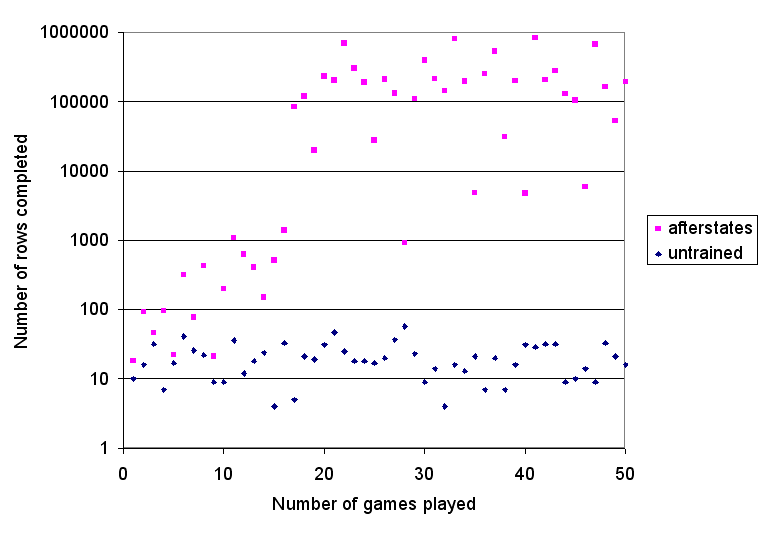
\includegraphics[width=3.5in]{afterstatesredtet4well.png}
\caption{TD(0) agent in well of width 4}
\label{fig:afterstatesredtet4well}
\end{figure}

The TD(0) agent performs well in a reduced well four blocks wide. After 19 games the performance jumps two orders of magnitude and the agent proceeds to complete over 100 000 rows the majority of the time, and nearly a million rows on occasion.

This explosive jump in performance could be due to two factors. The most obvious is that the agent may have discovered a significant series of improvements to its policy. What is less obvious is that the agent learns after every single move, so the longer the agent survives the more the agent learns and a self sustaining cycle of survival and learning is achieved.

\begin{figure}[h]
\centering
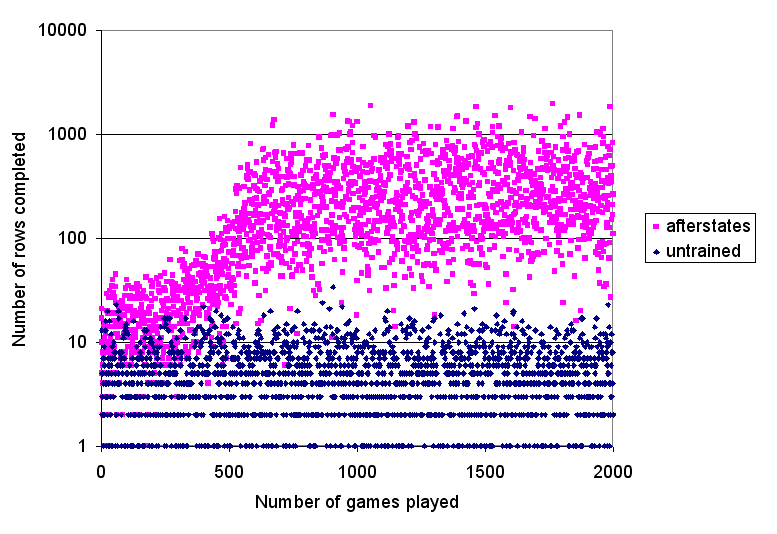
\includegraphics[width=3.5in]{afterstatesredtet5well.png}
\caption{TD(0) agent in well of width 5}
\label{fig:afterstatesredtet5well}
\end{figure}

As the width is increased the performance of the agent deteriorates drastically. With a well width of 5 the agent takes about 700 games to discover the optimal policy, which results in the agent completing around 300 rows per game.

When observing the agent playing there were some obvious shortcomings to be seen in the TD(0) agent's tactics. The agent was oblivious to the introduction of holes and introduced them liberally in trying to achieve immediate rewards. This is not suprising considering the contour representation we adopted, which is oblivious to anything beneath the top layer of the well. 

We tried to correct for this by adopting a real time penalty for introducing covered holes. This created the problem of weighting the hole penalty against the row completion reward. The problem was further aggravated by the fact that introducing holes does not have uniform impact. In some circumstances introducing a hole has little impact, and in others it can completely negate the value of the transition. This is best shown with the L block from the standard tetromino set and is shown in figure \ref{fig:diffholes}. 

\begin{figure}[h]
\centering
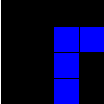
\includegraphics[width=1in]{worthless.png}
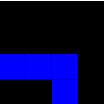
\includegraphics[width=1in]{notworthless.png}
\caption{Contrasting hole inclusion}
\label{fig:diffholes}
\end{figure}

The introduction of two vertical holes has a far more damaging effect than introducing two horizontal holes as it effects two separate rows. In introducing the two horizontal holes the L block has also extended across three quarters of the reduced well, which places the agent in a position where it will most likely receive a reward in the next transition.

\section{Sarsa($\lambda$) agent}

The performance of the Sarsa($\lambda$) agent is shown for wells of width 4 and 5 in figures \ref{fig:sarsaeligredtet4well} and \ref{fig:sarsaeligredtet5well}.

\begin{figure}[h]
\centering
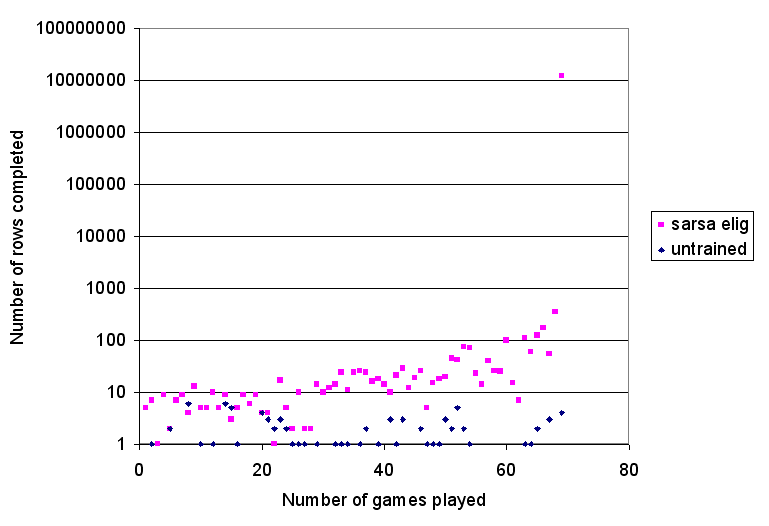
\includegraphics[width=3.5in]{sarsaeligredtet4well.png}
\caption{Sarsa agent in well of width 4}
\label{fig:sarsaeligredtet4well}
\end{figure}

The Sarsa($\lambda$) agent performs incredibly in the 4 block wide well. Although the Sarsa($\lambda$) agent takes longer to train then the TD(0) player, the performance explosion that occurs at around 76 games is unparallelled. The agent was left to play for a day and had to be forcibly terminated in order to end the game and free up the computer it was running on. Figure \ref{fig:sarsaelig4term} shows the game at the time of termination 

\begin{figure}[h]
\centering
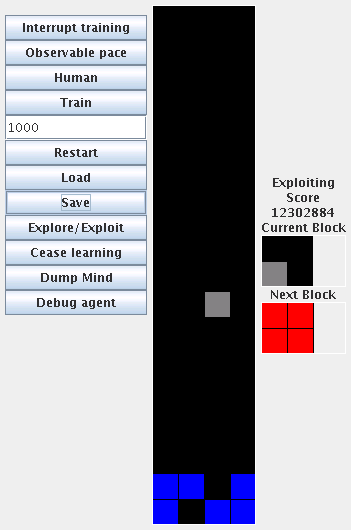
\includegraphics[width=2in]{sarsaelig4term.png}
\caption{Sarsa agent at time of termination}
\label{fig:sarsaelig4term}
\end{figure}

\begin{figure}[h]
\centering
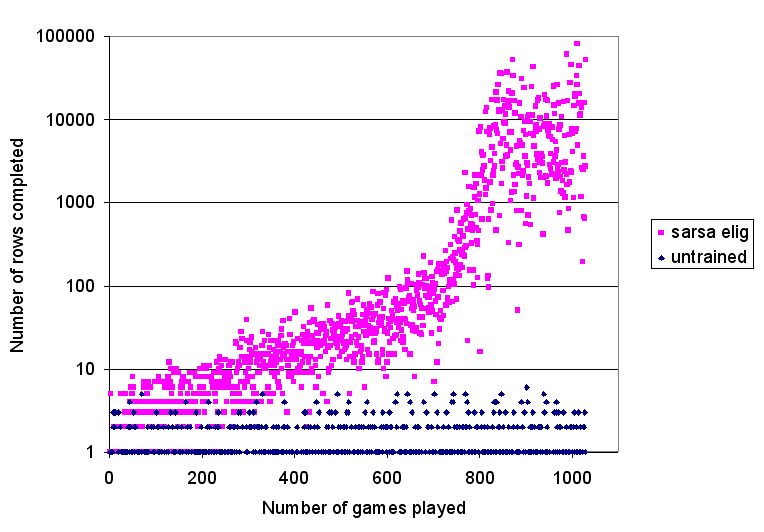
\includegraphics[width=3.5in]{sarsaeligredtet5well.png}
\caption{Sarsa agent in well of width 5}
\label{fig:sarsaeligredtet5well}
\end{figure}

The Sarsa($\lambda$) agent in a well of width 5 shows steady improvement over the course of its lifespan. Somewhere around 700 games the rate of improvement increases and the agent reaches the optimal policy at around 900 games. At this point the agent is capable of completing around 10 000 rows per game.

The Sarsa($\lambda$) agent displays very different in-game tactics to the TD(0) agent. The player places blocks intelligently, and creates a solid well structure. This is due to the fact that the agent is aware of introducing holes, and the associated penalty is incorporated in the relative state-action transition.

The drop in performance that becomes evident in the altering of the well size may be due to qualities associated with the well rather short comings on the part of the agent. There is no mathematical proof guaranteeing the termination of the Tetris game when using the reduced tetromino set and there are no obvious combinations of tetrominoes that would be terminal in the well of width 4. On the other hand a sequence of square tetrominoes in the well of width 5 would completely overwhelm the agent, and increase the height of the well structure failing it actually killing the agent. This may well account for the wider agents inability to play indefinitely like the agent learning in the well of width 4.

\section{Conclusion}

We implemented TD(0) and Sarsa($\lambda$) agents, and investigated the performance of the agents as the wells they function in are widened. 

\chapter{Full Tetris}

In this chapter we extend our contour agents to play in the full Tetris well and investigate several side effects of this extension.

\section{Results}

The two competing methods responsible for bridging the semantic gap between the subwells and full well were investigated using the Sarsa($\lambda$) agent.

\begin{figure}[h]
\centering
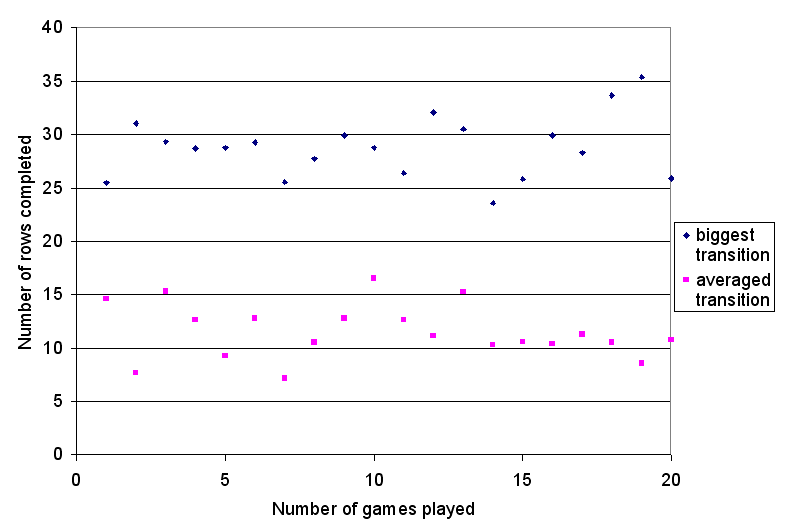
\includegraphics[width=3.5in]{multisingle.png}
\caption{Contrast between selecting biggest transition and taking the average of the transitions}
\label{fig:multisingle}
\end{figure}

The results for both methods are incredibly noisy. It warrants mentioning that the agent is exploiting its knowledge at this point and that no further learning is occurring. The variance is therefore due to the tetrominoes assigned to the agent, and the order in which the agent receives them.

The results achieved by taking the biggest transition seemed to consistently beat the results achieved by the averaging method. This came as some suprise as we expected the averaging approach to give a more accurate reflection of the true value of a transition. In retrospect the averaging of the transitions results in a value that is not really representative of anything. An action that is fair in all subwells will possibly be selected over an action that is predicted to be both incredible and terrible in different subwells.

The biggest subwell transition was used within the full well in all subsequent investigations. 

The size of the subwell the agent was trained in was predicted to have an impact on the performance of the agent in the full game. This extendability of different width subwells was investigated using the Sarsa($\lambda$) agent and the results are shown in figures \ref{fig:widthcomparrison} and \ref{fig:widthcomparrisonfulltet}.

\begin{figure}[h]
\centering
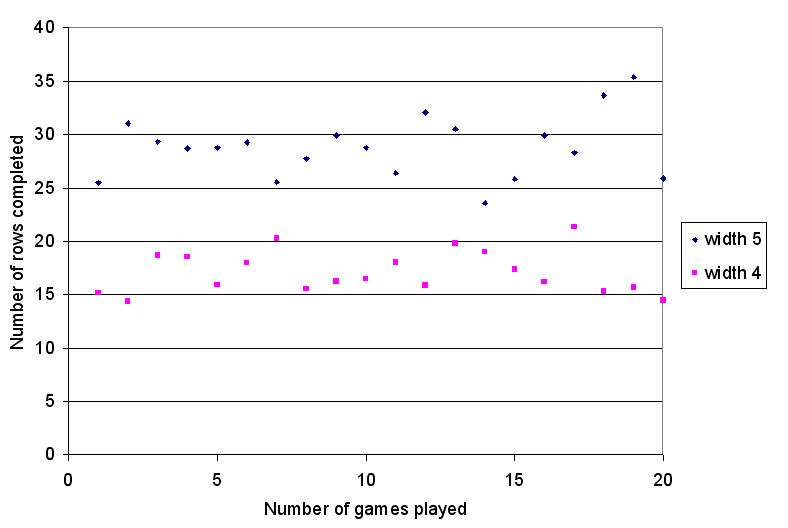
\includegraphics[width=3.5in]{widthcomparrison.png}
\caption{Comparison of extendability of subwell sizes with reduced tetrominoes}
\label{fig:widthcomparrison}
\end{figure}

\begin{figure}[h]
\centering
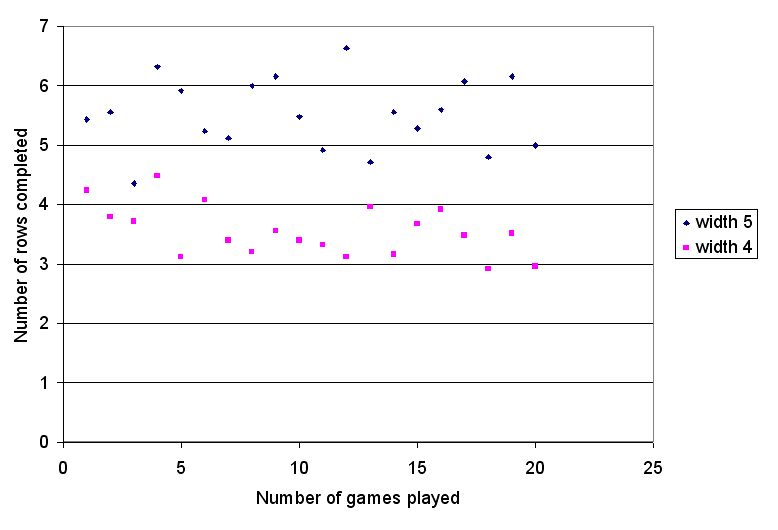
\includegraphics[width=3.5in]{widthcomparrisonfulltet.png}
\caption{Comparison of extendability of subwell sizes with standard tetrominoes}
\label{fig:widthcomparrisonfulltet}
\end{figure}

Both investigations revealed a distinct advantage to the player trained within a well of width 5.

Although the final state space design was chosen to represent a well four blocks wide, agents trained in narrow wells developed a policy which favoured easy returns. In narrow wells there is a rapid turnover of rows since 2 blocks on average complete a row. Introducing holes therefore has minor implications as rows have a short lifespan and the obstructing layer is likely to removed in the ensuing block placements. This performance does not scale out to the full representation of the game, where a single introduced hole can devalue a series of successive compact placements and have long term implications.

By extending the width of the reduced well the agent trains within a broader well and tends towards a policy that reflects the policy required in playing the game. We narrowed the well in order to reduce the state space, and every extra unit of width increases the state space by a factor of seven for our contour representation. We therefore seek to strike a balance between increasing the state space and giving the agent access to the environment we want him to eventually solve.

The final agents adopted were therefore all trained in a well of width five.

The remaining experimention requires the direct comparison of the the TD(0) and Sarsa($\lambda$) agent. The agents were initially set to use the reduced tetromino set and are compared in figures \ref{fig:afterstatesredtetfullwell} and \ref{fig:sarsaeligredtetfullwell}.

\begin{figure}[h]
\centering
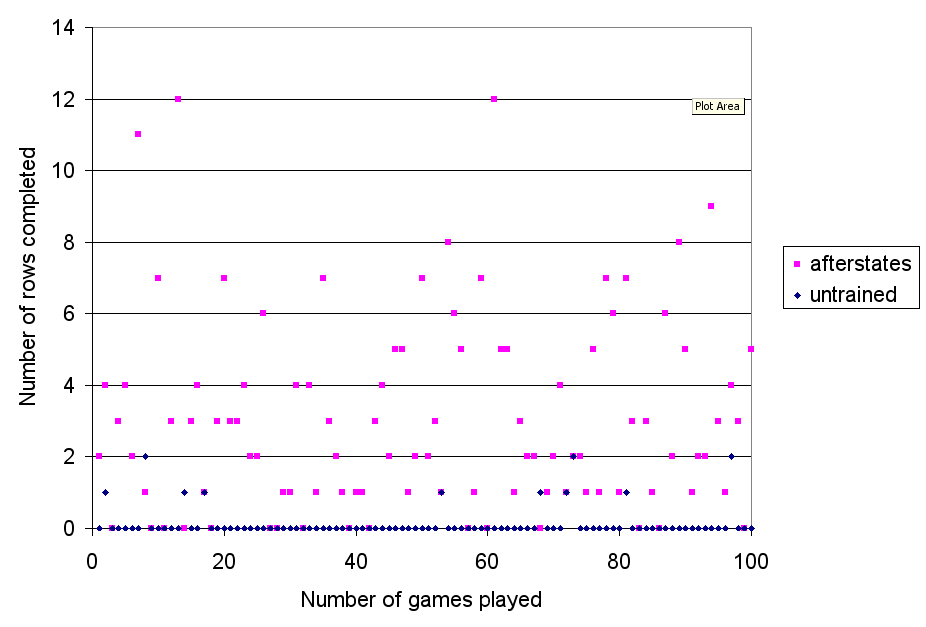
\includegraphics[width=3.5in]{afterstatesredtetfullwell.png}
\caption{TD(0) agent in full well with reduced tetrominoes}
\label{fig:afterstatesredtetfullwell}
\end{figure}

\begin{figure}[h]
\centering
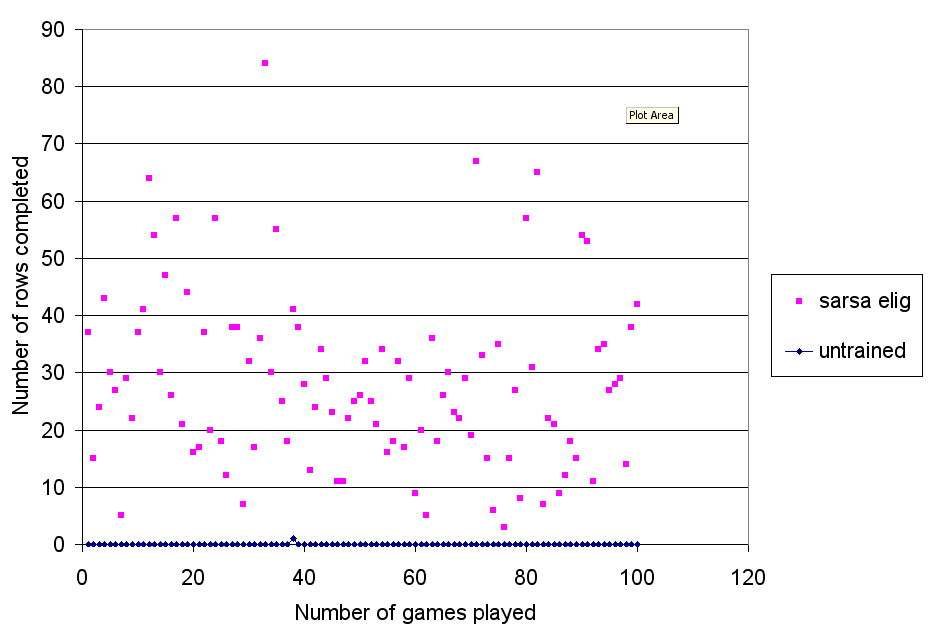
\includegraphics[width=3.5in]{sarsaeligredtetfullwell.png}
\caption{Sarsa agent in full well with reduced tetrominoes}
\label{fig:sarsaeligredtetfullwell}
\end{figure}

\begin{figure}[h]
\centering
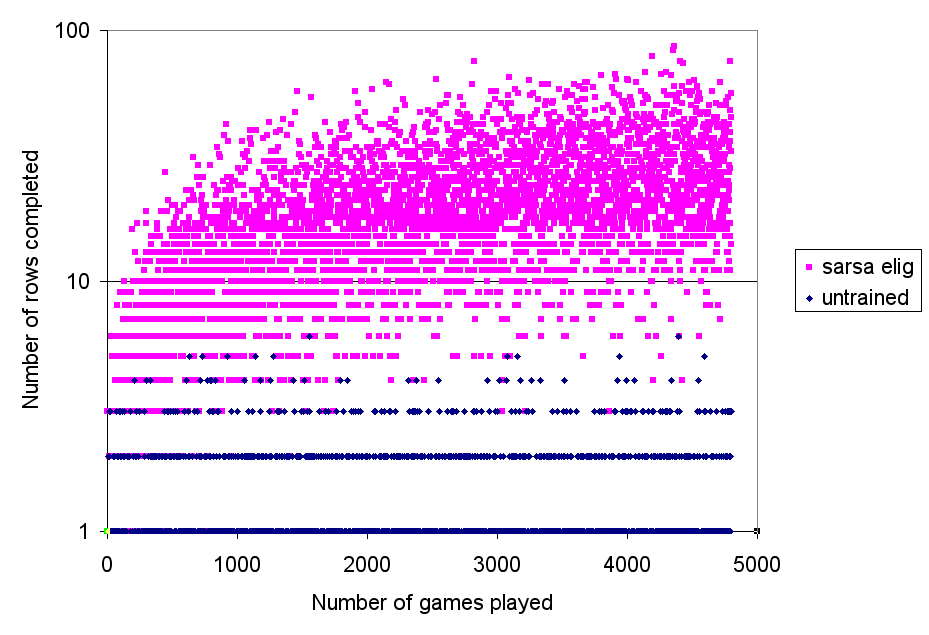
\includegraphics[width=3.5in]{sarsaeligfulltetredwell.png}
\caption{Sarsa agent in reduced well with full tetrominoes}
\label{fig:sarsaeligfulltetredwell}
\end{figure}

\begin{figure}[h]
\centering
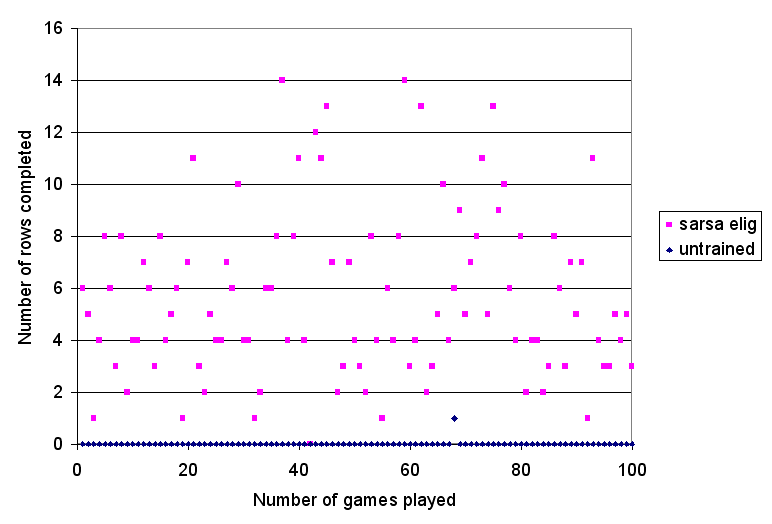
\includegraphics[width=3.5in]{sarsaeligfulltetfullwell.png}
\caption{Sarsa agent in full well with full tetrominoes}
\label{fig:sarsaeligfulltetfullwell}
\end{figure}

\begin{figure}[h]
\centering
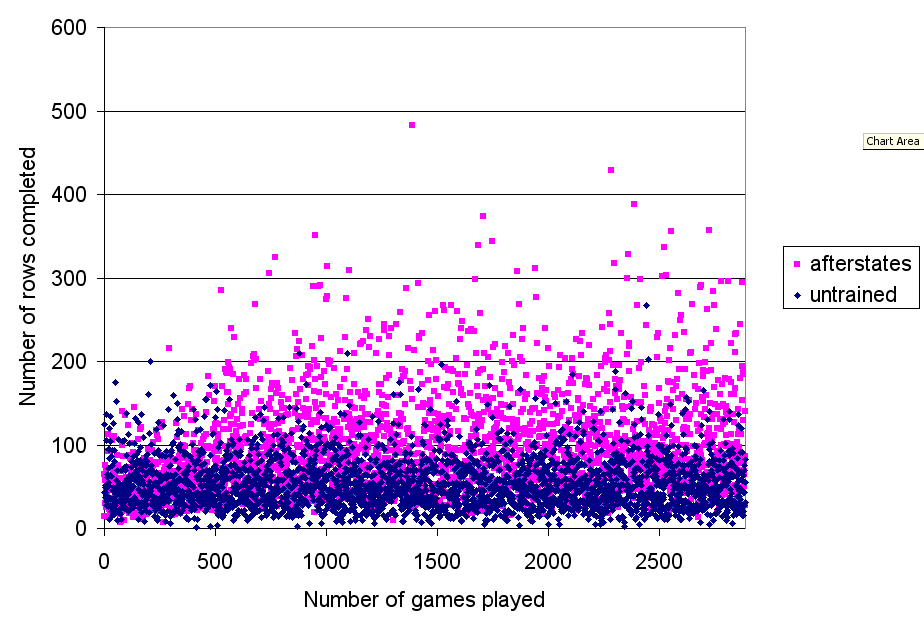
\includegraphics[width=3.5in]{afterstatesheightredtetfullwell.png}
\caption{TD(0) agent in full well with red tetrominoes}
\label{fig:afterstatesheightredtetfullwell}
\end{figure}

\section{Conclusion}

In this chapter we extended our contour agents to play in the full Tetris well.

\chapter{Concluding remarks}

The TD(0) agent achieved incredible results when playing within the original subwell. These results were unrealistically high, and dropped off sharply as the well was increased and real time rewards became more intermittent. The TD(0) representation neglected the importance of different transitions.

The Sarsa($\lambda$) player achieved incredible results within the original subwell defined in the state space reduction. The performance was still impressive as the well width was increased, although the required training time greatly increased.

The reducing of the state representation had a greater impact on the TD(0) approach, since this approach depends purely on the accuracy of the state information. The extended resolution afforded the Sarsa($\lambda$) player enabled it to associate a value with the act of transitioning off a state. 

\bibliography{finalwriteup}

\end{document}
